%!TEX program = xelatex
%!TEX TS-program = xelatex
%!TEX encoding = UTF-8 Unicode

\documentclass[12pt, a4paper]{article} % A4 纸,字体大小为 12pt 的 article 类文档
\usepackage{CJKutf8} % 中文支持
\usepackage{graphicx} % 插入图片
\usepackage{subfigure} % 插入多图时用子图显示的宏包
\usepackage{listings} % 支持代码显示
\usepackage{hyperref} % 超链接
\usepackage{ulem} % 删除线
\usepackage{xcolor} % 定制颜色
\usepackage{caption2} % 浮动图形和表格标题样式
\usepackage{amssymb} % 数学符号
\usepackage{graphicx} % 插入图片
% \usepackage{indentfirst} % 中文段落首行缩进
\setlength{\parindent}{0pt} % 设置段落缩进为 0
\usepackage{tikz} % 画图
\usepackage{pgfplots} % 画图
\usepackage{amsmath} % 处理数学公式
\usepackage{mathtools} % 处理数学公式
\usepackage{setspace}
\usepackage{url}
\usepackage[english]{babel}
\usepackage{booktabs}
\usepackage{fancyvrb} % 导言区添加 fancyvrb 宏包
\setlength{\parskip}{0.5em} % 段落间距
% \setstretch{1.2} % 设置行间距
\renewcommand{\figurename}{图} % 将图的标题设置为中文“图”
\renewcommand{\tablename}{表} % 将表的标题设置为中文“表”
\renewcommand{\lstlistingname}{代码} % 更改代码块标题的名称为 "代码"
\usetikzlibrary{tikzmark,calc,decorations.pathreplacing} % tikzmark 用于标记位置,calc 用于计算,decorations.pathreplacing 用于画大括号
\lstset{
    % backgroundcolor=\color{white!70!yellow}, % 背景色为浅黄色
    frame=single,
    breaklines=true, % 自动折行
    postbreak=\mbox{\textcolor{red}{$\hookrightarrow$}\space} % 折行后添加箭头符号
}

\hypersetup{
    colorlinks=true,
    linkcolor=blue,
    urlcolor=blue,
    citecolor=blue
}

\title{nginx笔记}
\author{hoochanlon}
\date{\today}

\begin{document}
\begin{CJK*}{UTF8}{gbsn}
\maketitle

\clearpage
\section{nginx.conf 入门配置}
\subsection{配置文件结构}
nginx配置为 /etc/nginx/nginx.conf,删除nginx.conf,并从零开始新建配置文件,代码如下:

\begin{lstlisting}[language=bash]
user root;
worker_processes 1;
events{
    worker_connections 1024;
}
http{
     server{
      location /{
        root /data/www;
    }
    location /images/ {
        root /data;
        }
    }
}
\end{lstlisting}

通过~ \verb|mkdir -p /data/www /data/images|~,以及简单创建~index.html~与测试图片,放入~/data/www~与~/data/images~,然后~\verb|nginx -s reload|~,
我们访问~http://localhost/~就可以看到~index.html~的页面效果,以及访问~http://localhost/images/test.jpg~显示图片。

\subsection{遇到过的错误}

错误如下:
\begin{lstlisting}[language=bash]
nginx: [error] open() "/run/nginx.pid" failed (2: No such file or directory)
\end{lstlisting}
解决办法:通过检查~\verb|/run|~ 目录是否存在,是否具备读写和执行权限,并以此进行相关操作,然后重启~nginx~即可。
\begin{lstlisting}[language=bash]
ls /run
sudo chmod 755 /run
sudo systemctl restart nginx
\end{lstlisting}

\subsection{基础开关命令}

分别是重载、停止、正常退出。
\begin{lstlisting}[language=bash]
nginx -s reload
nginx -s stop
nginx -s quit
\end{lstlisting}

\subsection{nginx~进程模型}
nginx~接收到~\verb|nginx -s reload|~后,~master~进程将启动新的~worker~进程,并向旧的~worker~进程发送信号,让其优雅退出;意外情况就是回滚操作,让其继续使用旧的~worker~进程。\par

~master~进程主要是负责读取和评估,并维护~worker~进程;微观上来看,即控制命令。~worker~进程主要是负责处理请求,以及响应请求;从微观的角度,即核心任务,请求转发、反向代理、负载均衡等工作。\par

~nginx~采用事件驱动机制,会给各个worker进程分配有效请求,~worker~进程默认数量为可用CPU内核数。\par

\renewcommand{\figurename}{图} % 将图表的标题设置为中文“图”
\begin{figure}[htbp]
    \centering
    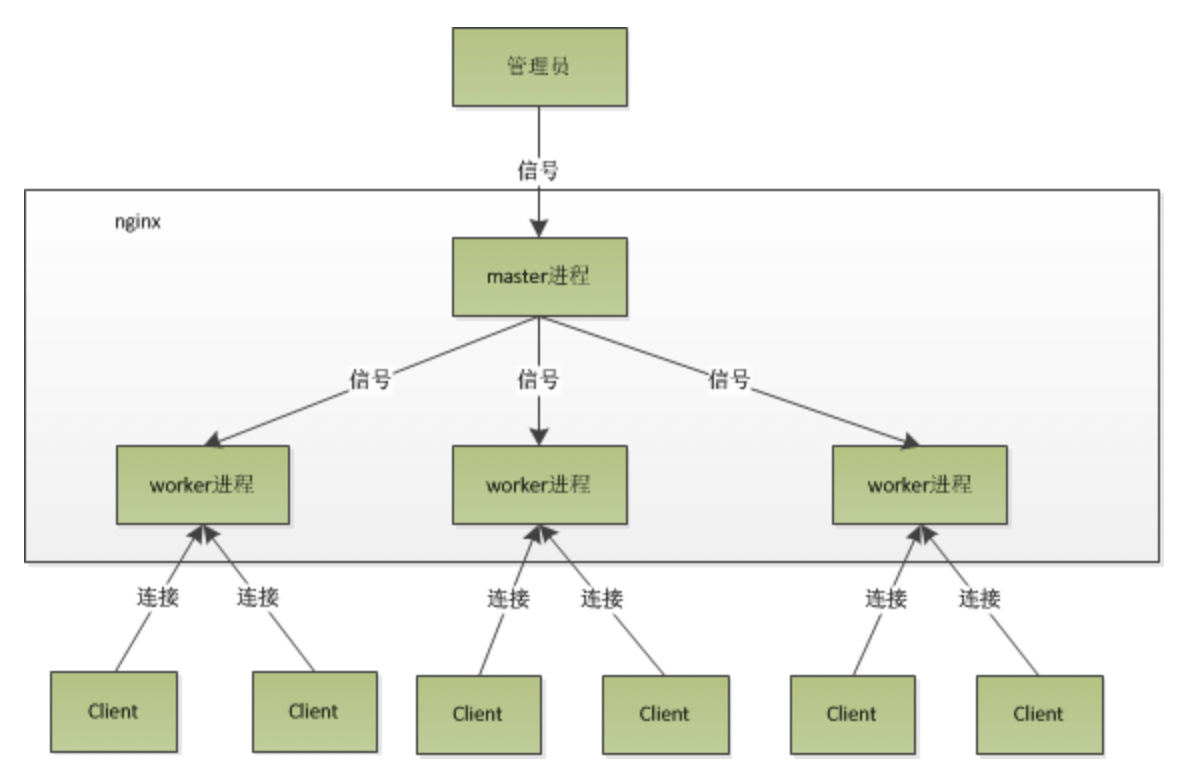
\includegraphics[width=1\textwidth]{./imgs/catch2023-08-19-10.37.16.png}
    \caption{~nginx~进程结构}
\end{figure}

\subsection{nginx~进程具体行为}

\[
    \text{master}
    \begin{cases}
         \text{读取并验证配置文件,以及重启配置文件。}   \\\\
         \text{创建、绑定和关闭套接字。} \\\\
         \text{启动、停止、维护特定的worker进程,以及相关进程升级。} \\\\
         \text{重新打开日志文件。} \\\\
         \text{动态加载第三方模块。} \\\\
         \text{worker}\left\{
            \begin{aligned}
                &\text{处理并发连接请求。}  \\\\
                &\text{提供反向代理和内容过滤功能。} \\\\
                &\text{实现~nginx~提供的其余所有功能(如安全与访问控制)。}
            \end{aligned}
            \right. \\
    \end{cases}
\]

\subsection{nginx~进程模型相关优点的思考}

引述\href{https://aceld.gitbooks.io/nginx-zh/content/31_nginxjin_cheng_mo_xing.html}{~aceld-~Nginx~进程模型~}做为分析:

\begin{enumerate}
    \item 对于每个worker进程来说,独立的进程,不需要加锁,所以省掉了锁带来的开销,同时在编程以及问题查找时,也会方便很多。
    \item 采用独立的进程,可以让互相之间不会影响,一个进程退出后,其它进程还在工作,服务不会中断,master进程则很快启动新的worker进程。
    \item 如果worker进程的异常退出,肯定是程序有bug了,异常退出,会导致当前worker上的所有请求失败,不过不会影响到所有请求,所以降低了风险。
\end{enumerate}

从~ChatGPT~中得知,共享内存需要加锁的原因是保持数据读写的一致性,防止相互覆盖,导致数据不一致的问题。


\clearpage
\section{架构设计与工作模式}
\subsection{模块路径及体系}
在默认情况下,Nginx 的模块位于 Nginx 的安装目录下的 modules 子目录中。具体路径可能会因操作系统的不同,存在路径上的差异。

\begin{figure}[htbp]
    \centering
    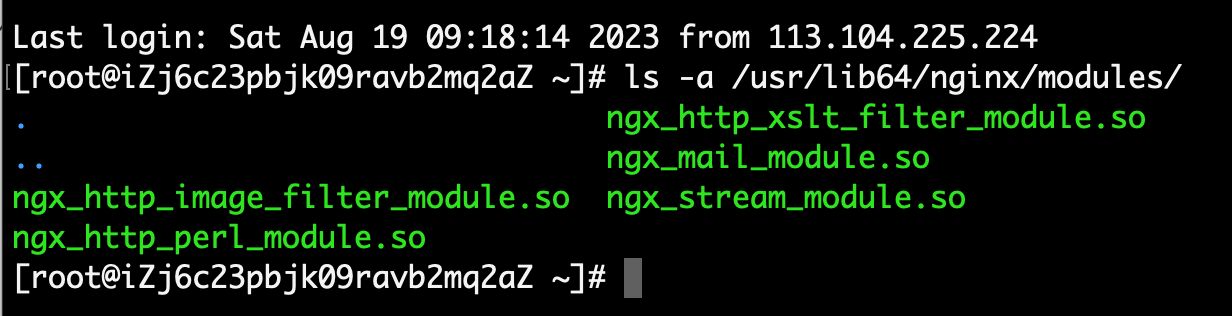
\includegraphics[width=0.9\textwidth]{./imgs/catch2023-08-19-16.28.04.png}
    \caption{~nginx~模块内容}
\end{figure}

这些模块可以按照功能进行分类:核心功能、事件处理、阶段处理(HTTP模块、mail模块、部分第三方模块)等。

\begin{figure}[htbp]
    \centering
    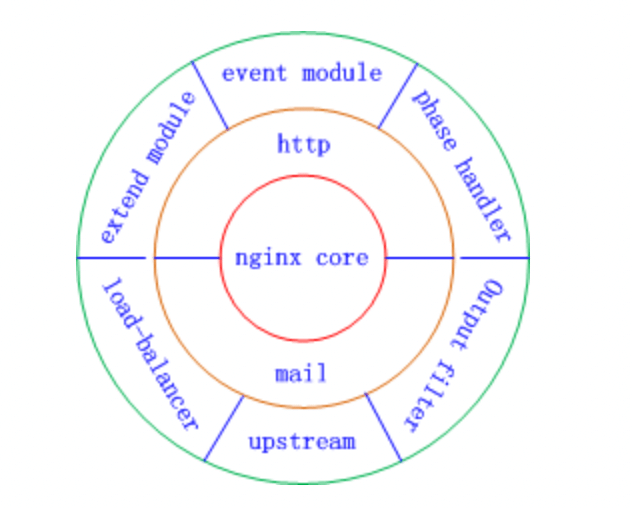
\includegraphics[width=0.8\textwidth]{./imgs/catch2023-08-19-16.16.15.png}
    \caption{~nginx~模块体系}
\end{figure}

\subsection{nginx的工作模式}
在具有多核~CPU~的环境下,NGINX~通常启动多个~worker~进程,每个进程都可以分配到一个~CPU~核心上运行。这样做有助于充分利用多核~CPU~的并行计算能力。\par

关于物理存储设备的使用效率,NGINX~采用异步非阻塞的事件驱动模型,在处理请求时能够有效地利用物理存储设备(如磁盘)的读写能力。每个~worker~进程可以独立处理请求,
如果其中一个进程需要进行磁盘操作(如读取文件),它可以执行该操作而不会阻塞其他进程的执行,从而提升了物理存储设备的使用效率。 \par

总结起来,多个~worker~进程可以充分利用多核~CPU~的并行计算能力,同时通过异步非阻塞的事件驱动模型,提升了物理存储设备的使用效率。这样可以更高效地处理请求,
减少资源竞争和阻塞等问题,提升系统性能和响应速度。

\begin{itemize}
    \item CPU~密集型:处理大量协议请求,或执行压缩等。(~CPU~配置)
    \item I/O~密集型:处理大量静态文件,执行磁盘缓存等。(磁盘配置)
\end{itemize}

\subsection{事件驱动模型}

参考 \href{https://www.cnblogs.com/crazymakercircle/p/15411888.html}{~Nginx 事件驱动模型~},事件驱动模型一般是由事件收集器,事件发送器,
事件处理器三部分基本单元组成。基于事件驱动模型可以有以下几种实现办法:

\begin{enumerate}
    \item “事件发送器”每传递过来一个请求,“目标对象”就创建一个新的进程,调用“事件处理器”来处理该请求。
    \item “事件发送器”每传递过来一个请求,“目标对象”就创建一个新的线程,调用“事件处理器”来处理该请求。
    \item “事件发送器”每传递过来一个请求,“目标对象”就将其放入一个待处理事件的列表,使用非阻塞I/O方式调用“事件处理器”来处理该请求。
\end{enumerate}

将事件模型进行归纳:

\[
    \text{库}
    \begin{cases}
         \text{select}\left\{
            \begin{aligned}
                &\text{分别创建收集读事件、写事件和异常事件的描述符集合}   \\
                &\text{调用底层提供的select()函数,等待事件发生。} \\
                &\text{轮询所有事件描述符集合,如果有就处理} \\
            \end{aligned}
            \right. \\\\
            \text{poll}\left\{
                \begin{aligned}
                    &\text{创建一个收集读事件、写事件和异常事件的描述符集合}   \\
                    &\text{分别为描述符分配对应事件。} \\
                    &\text{同时检查三种情况是否发生。} \\
                \end{aligned}
                \right. \\\\
            \text{epoll}\left\{
                \begin{aligned}
                    &\text{通知内核创建一个由N个描述符的事件列表。}   \\
                    &\text{给这些描述符设置所关注的事件,并添加到内核的事件列表。} \\
                    &\text{内核把发生事件的描述符列表通知给进程,避免了轮询。} \\
                \end{aligned}
                \right. \\
    \end{cases}
\]

再结合 \href{https://blog.51cto.com/yyxianren/5721144}{51cto - nginx架构分析之事件驱动模型}文章提供的分析图

\begin{figure}[htbp]
    \centering
    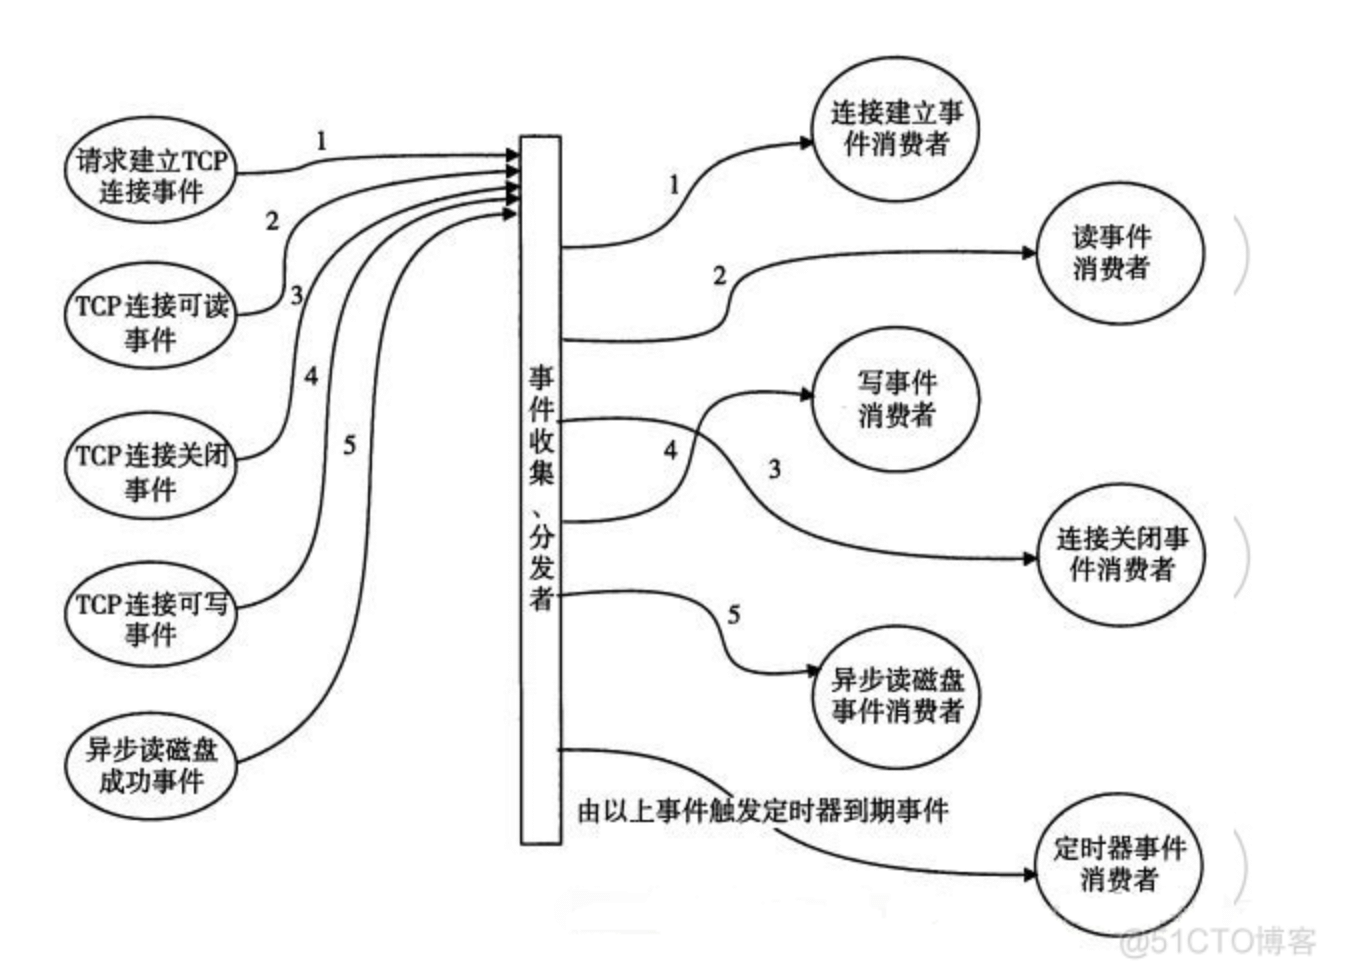
\includegraphics[width=0.8\textwidth]{./imgs/catch2023-08-19-19.18.04.png}
    \caption{~nginx~事件驱动模型}
\end{figure}

由此我们就对nginx的结构设计与工作机制,以及其事件驱动模型有了较为基础的认识。


\clearpage
\section{nginx 目录结构}
\subsection{安装目录说明(部分)}

作用参考:\href{https://www.cnblogs.com/kai-/p/12810051.html}{cnblogs - CGI, FastCGI, WSGI, uWSGI, uwsgi一文搞懂}

\renewcommand{\tablename}{表}
\begin{table}[htbp]
    \centering
    \caption{示例表格}
    \begin{tabular}{ccc}
      \toprule
      路径 & 类型 & 作用 \\
      \midrule
      /etc/nginx/fastcgi\_params &  &  \\
      /etc/nginx/uwsgi\_params & 配置文件 & 通用网关接口,即中间件 \\
      /etc/nginx/scsgi\_params &  & \\
      \bottomrule
    \end{tabular}
  \end{table}

作用参考:\href{https://blog.csdn.net/wzj_110/article/details/112850811}{csdn~-~Nginx(十八)mime.types的作用}

\renewcommand{\tablename}{表}
\begin{table}[htbp]
    \centering
    \caption{示例表格}
    \begin{tabular}{ccc}
      \toprule
      路径 & 类型 & 作用 \\
      \midrule
      /etc/nginx/mime.type & 配置文件 & 定义文件类型操作方式 \\
      \bottomrule
    \end{tabular}
  \end{table}

作用参考:\href{http://www.ruanyifeng.com/blog/2016/03/systemd-tutorial-commands.html}{阮一峰~-~Systemd 入门教程:命令篇}

\renewcommand{\tablename}{表}
\begin{table}[htbp]
    \centering
    \caption{示例表格}
    \begin{tabular}{ccc}
      \toprule
      路径 & 类型 & 作用 \\
      \midrule
      /usr/lib/systemd/system/nginx-debug.service &  &  \\
/usr/lib/systemd/system/nginx.service & 配置文件 & 守护进程管理 \\
/etc/sysconfig/nginx &  & \\
/etc/sysconfig/nginx-debug &  & \\
      \bottomrule
    \end{tabular}
  \end{table}

\subsection{其他}

\verb|nginx -t -c /etc/nginx/nginx.conf| 用于测试~Nginx~配置文件的语法是否正确。

\verb|tail -f /var/log/nginx/error.log| 用于实时查看~Nginx~错误日志文件的最新内容(文件尾)。

\verb|ab -n 50 -c 20 http://116.62.103.228/index.html|  -n 50~执行50个请求,-c 20~并发20个请求。

% \subsection{nginx变量}
% 参考:https://victorfengming.gitee.io/file/pdf/tuling/Nginx面试题23道.pdf
% 参考:https://xuexb.github.io/learn-nginx/example/error-page.html nginx教程示例

\clearpage
\section{~nginx~模块练习与使用}

参考:\href{https://www.cnblogs.com/guarderming/p/10219661.html}{博客园-~Nginx~模块说明}

\subsection{stub\_status 查看~Nginx~的客户端状态}

一、通过向 \verb| etc/nginx/nginx.conf | 中加入

\begin{lstlisting}
location /mystatus{
    stub_status;
}
\end{lstlisting}

二、再通过 http://localhost/mystatus 访问,得到结果。

\begin{lstlisting}
Active connections: 1
server accepts handled requests
 4 4 5
Reading: 0 Writing: 1 Waiting: 0
\end{lstlisting}

Active connections 表示nginx活跃的连接数 \\\\
server accepts handled requests
\begin{enumerate}
    \item 第一个整数表示nginx处理握手的总次数。
    \item 第二个整数表示nginx处理的连接数。
    \item 第三个整数表示nginx处理的总的请求数。
\end{enumerate}
Waiting: ~0~表示~nginx~开启了常连接的情况下,客户端和服务端正在空闲的等待,既没有读也没有写,建立连接的数量。

\subsection{random\_index 设置随机网页}

先把网页样例的压缩文件拷贝到服务器。

\begin{lstlisting}
scp ./exam/exam_htmls.zip root@8.217.129.210:$HOMEPATH
\end{lstlisting}

然后在服务器端解压缩至接下来要配置的目录。

\begin{lstlisting}
mkdir -p /data
unzip -q exam_htmls.zip -d /data
\end{lstlisting}

配置文件

\begin{lstlisting}
location / {
    root /data/exam_htmls;
    random_index on;
}
\end{lstlisting}

\verb|systemctl reload nginx| 重启nginx服务,然后访问~http://localhost~,会发现每次访问的页面都不一样。

\subsection{更多模块使用方式}

\begin{itemize}
    \item ~nginx~第三方模块收集:\url{https://www.nginx.com/resources/wiki/modules/}
    \item ~nginx~中常用的模块整理1:\url{https://blog.csdn.net/qq_37510195/article/details/130532089}
    \item ~nginx~中常用的模块整理2:\url{https://blog.csdn.net/L596462013/article/details/131113768}
    \item ~nginx~官网模块教程:\url{https://nginx.org/en/docs/http/ngx_http_core_module.html}
\end{itemize}

\subsection{~nginx~访问控制}
nginx访问控制主要有两种:
\begin{enumerate}
    \item 基于IP的访问控制:http\_access\_module
    \item 基于用户的信任登录:http\_auth\_basic\_module
\end{enumerate}
这些功能都是基于模块化配置实现。

\clearpage
\section{~nginx~进阶大纲与问题联系}
\subsection{大纲}
\begin{enumerate}
    \item 静态资源~web~服务
    \item 代理服务
    \item 负载均衡调度器SLB
    \item 动态缓存
\end{enumerate}
\subsection{常见问题}
\begin{enumerate}
    \item 相同~server\_name~多个虚拟主机优先级访问
    \item ~location~匹配优先级
    \item ~try\_files~使用
    \item nginx~的~alias~和~root~的区别
    \item 用什么方法传递用户的真实IP
\end{enumerate}


\clearpage
\section{~nginx~静态资源访问}

\subsection{准备工作~·~理解代码}

观察以下代码:(具体可参考~\href{https://segmentfault.com/a/1190000020978410}{sf~-~nginx开启gzip压缩和静态缓存})
\begin{lstlisting}
server {
    listen       80;
    server_name  8.217.129.210;
    sendfile on;
    #charset koi8-r;
    access_log  /var/log/nginx/log/static_access.log  main;

location ~ .*\.(jpg|gif|png)$ {
    gzip on;
    gzip_http_version 1.1;
    gzip_comp_level 2;
    gzip_types text/plain application/javascript application/x-javascript text/css application/xml text/javascript application/x-httpd-php image/jpeg image/gif image/png;
    root /data/images;
}
location ~ .*\.(txt|xml)$ {
    gzip on;
    gzip_http_version 1.1;
    gzip_comp_level 1;
    gzip_types text/plain application/javascript application/x-javascript text/css application/xml text/javascript application/x-httpd-php image/jpeg image/gif image/png;
    root /data/docs;
}
    location ~ ^/download {
        gzip_static on;
        tcp_nopush on;
        root /data/files;
    }
}
\end{lstlisting}

设置gzip压缩针对的HTTP协议版本,没做负载的可以不用,一般设置为1.1保证兼容性。\\\\
设置gzip压缩级别,级别越高压缩率越高,但是消耗CPU资源也越多,设置为1,一般情况够用。\\\\
gzip\_types,设置需要压缩的MIME类型,如果不在设置类型范围内的请求不进行压缩。 \\\\
gzip\_static on,启用静态 gzip 压缩。当客户端发送请求时,如果服务器上存在经过预先压缩的 gzip 静态文件,Nginx 会直接返回该文件,提供更快的传输速度。\\\\
tcp\_nopush on,开启 tcp\_nopush 选项。该选项用于提高网络传输性能,当启用时,Nginx 会尽量将响应数据发送给客户端,而不是等待缓冲区填充满再发送。

\subsection{准备工作~·~Location~理解路由规则与conf.d配置}

首先做一下全局性的回顾:\href{https://www.cnblogs.com/knowledgesea/p/5175711.html}{cnblogs~-~Nginx配置详解}。之后细化到对路由规则配置的查阅:
\begin{itemize}
    \item \href{https://zhuanlan.zhihu.com/p/627557214}{知乎专栏~-~Nginx Location路由规则配置详解}。
    \item \href{http://unclezs.com/pages/65844e}{unclezs~-~Location路由规则配置详解}。
\end{itemize}

有时候我们安装了~nginx~后发现配置文件只有一个,/etc/nginx/nginx.conf。所有的配置包括虚拟目录也在此文件中配置, 这样当虚拟主机多了管理就有些不方便了,
这是需要我们把配置文件拆分开来。参考\href{https://www.cnblogs.com/fps2tao/p/9958009.html}{~cnblogs~-~增加nginx虚拟主机配置文件(conf.d)}。

\subsection{开始实践}

拷贝文件到服务器的测试目录(没有可自己着手创建,图片也是一样)。
\begin{lstlisting}
scp ~/test.img.gz root@8.217.129.210:/data/files
scp  ~/images/wei.png root@8.217.129.210:/data/images
scp ~/access.txt  root@8.217.129.210:/data/docs
\end{lstlisting}
然后根据6.1提供的代码,配置~vim /etc/nginx/conf.d/static\_server.conf~文件。并创建文件夹:

\begin{lstlisting}
# chmod 777 /var/log/nginx/log
sudo mkdir -p /var/log/nginx/log
\end{lstlisting}
测试,并启动
\begin{lstlisting}
nginx -tc /etc/nginx/nginx.conf
systemctl reload nginx
\end{lstlisting}
测试效果
\renewcommand{\figurename}{图} % 将图表的标题设置为中文“图”
\begin{figure}[htbp]
    \centering
    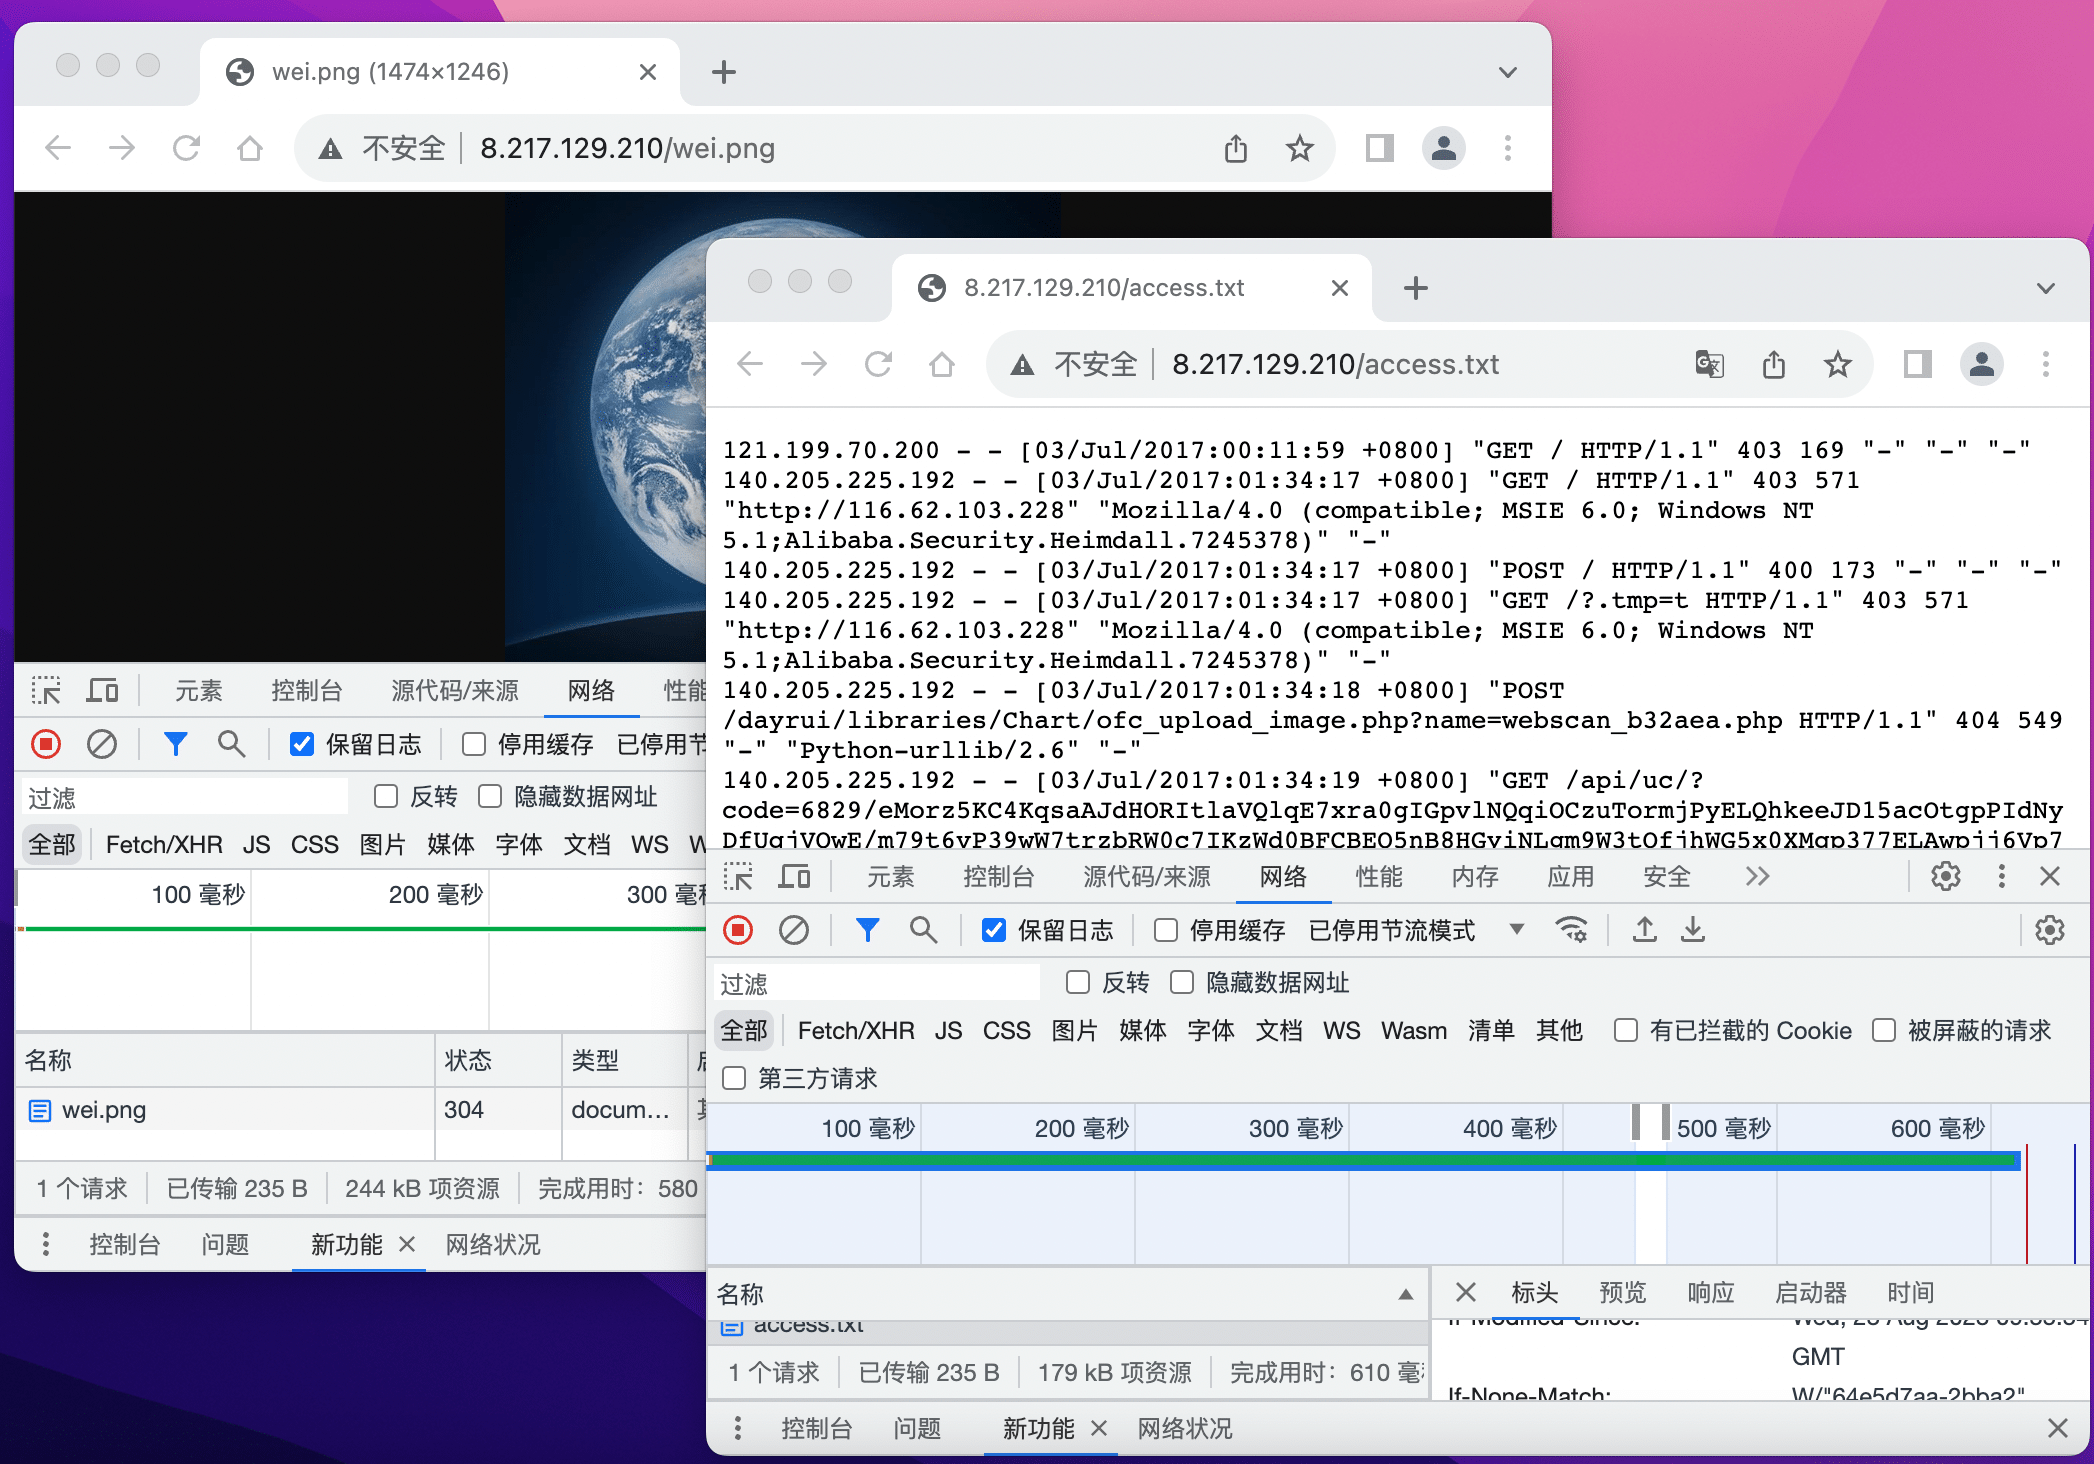
\includegraphics[width=1\textwidth]{./imgs/catch2023-08-23-18.09.54.png}
    \caption{~gzip~配置测试效果}
\end{figure}

\clearpage
\section{浏览器缓存}

\subsection{浏览器获取缓存的流程}
\renewcommand{\figurename}{图} % 将图表的标题设置为中文“图”
\begin{figure}[htbp]
    \centering
    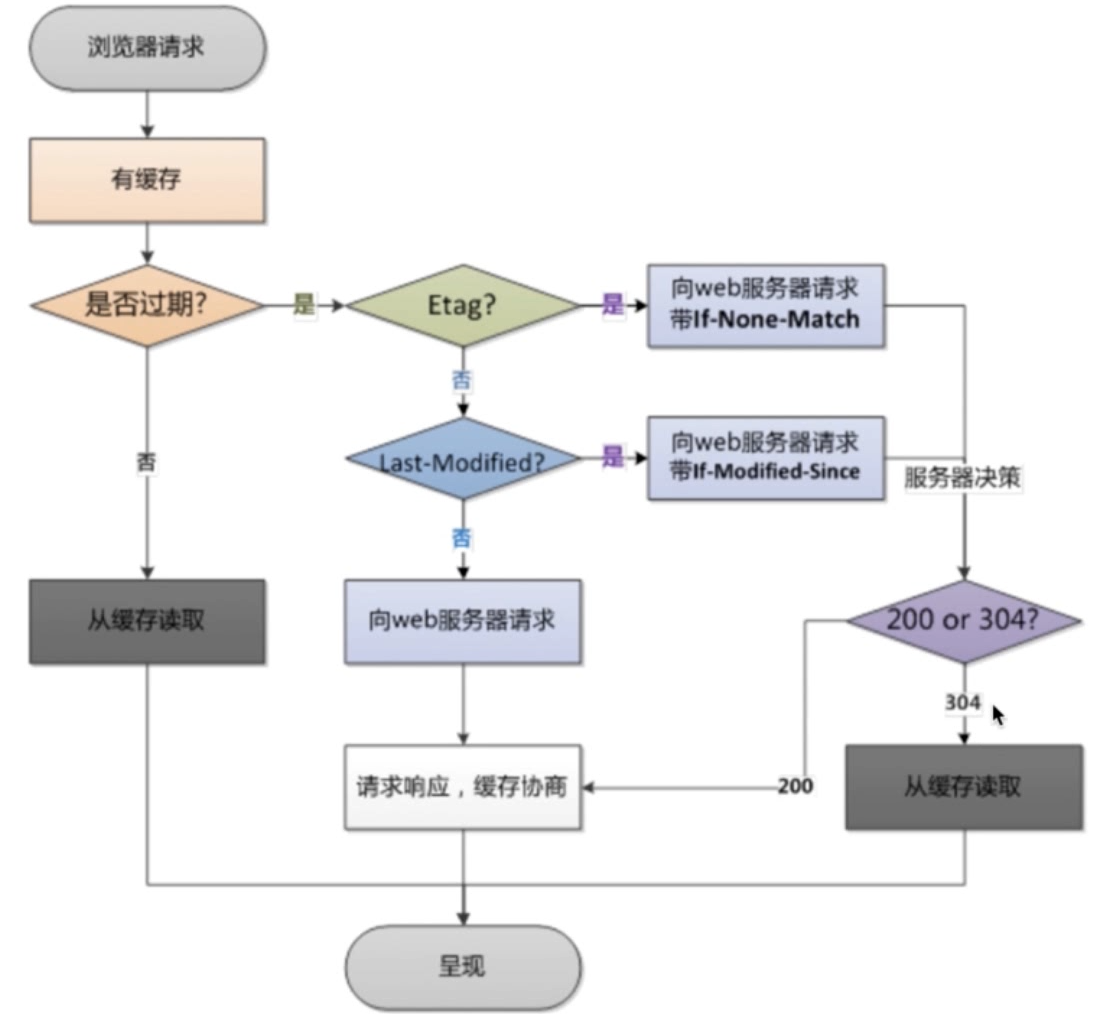
\includegraphics[width=1\textwidth]{./imgs/catch2023-08-23-18.30.26.png}
    \caption{~gzip~配置测试效果}
\end{figure}

\clearpage
\subsection{ETag}
ETag~是“实体标签”(Entity Tag)的缩写,是资源的一个唯一标识,主要是用来解决修改时间无法准确区分文件变化的问题。

比如,一个文件在一秒内修改了多次,但因为修改时间是秒级,所以这一秒内的新版本无法区分。再比如,一个文件定期更新,但有时会是同样的内容,
实际上没有变化,用修改时间就会误以为发生了变化,传送给浏览器就会浪费带宽。使用 ETag 就可以精确地识别资源的变动情况,让浏览器能够更有效地利用缓存。

参考 \href{https://www.codenong.com/cs105674287/}{码农家园-什么是Etag?}

\subsection{last-modified}
Last-Modified~是~HttpHeader~中的资源的最后修改时间,如果带有~Last-Modified ,下一次发送~Http~请求时,将会发生带~If-modified-since~的~HttpHeader~。
如果没有过期,将会收到304的响应,从缓存中读取。

参考 \href{https://blog.csdn.net/caseywei/article/details/108389859}{~csdn~-(转)缓存Last-Modified,Etag,Expire区别}

\subsection{附:防盗链设置参考}

\begin{lstlisting}
valid_referers 192.168.44.101;
    if ($invalid_referer) {
        return 403;
}
\end{lstlisting}

参考:\href{https://blog.csdn.net/weixin_46560589/article/details/126411063}{csdn~-~Nginx-防盗链}、
\href{https://blog.csdn.net/weixin_46560589/article/details/126411063}{csdn~-Nginx(七)防盗链}

\subsection{附:跨域访问}

在location块中加入以下代码,即可实现跨域访问。

\begin{lstlisting}
add_header Access-Control-Allow-Origin *;
add_header Access-Control-Allow-Methods GET,POST,OPTIONS;
\end{lstlisting}

参考:\href{https://blog.csdn.net/zhongxj183/article/details/123051546}{csdn~-~Nginx配置valid\_referer解决跨站请求伪造(CSRF)}、
\href{https://www.cnblogs.com/javasl/p/12862697.html}{cnblogs~-(011)Nginx静态资源web服务\_跨站访问}

\clearpage
\subsection{设置缓存开始实践}

time可以为正数,也可以为负数,默认单位为秒。

\begin{itemize}
    \item 如果为正数或0,则响应为:Cache-Control:max-age=time。
    \item 如果为负数,则响应为:Cache-Control:no-cache,即不缓存。
\end{itemize}

\begin{lstlisting}
location ~.*\.(htm|html)$ {
    #expires 24h;
    expires 10;
    root /data/www;
}
\end{lstlisting}

测试效果
\renewcommand{\figurename}{图} % 将图表的标题设置为中文“图”
\begin{figure}[htbp]
    \centering
    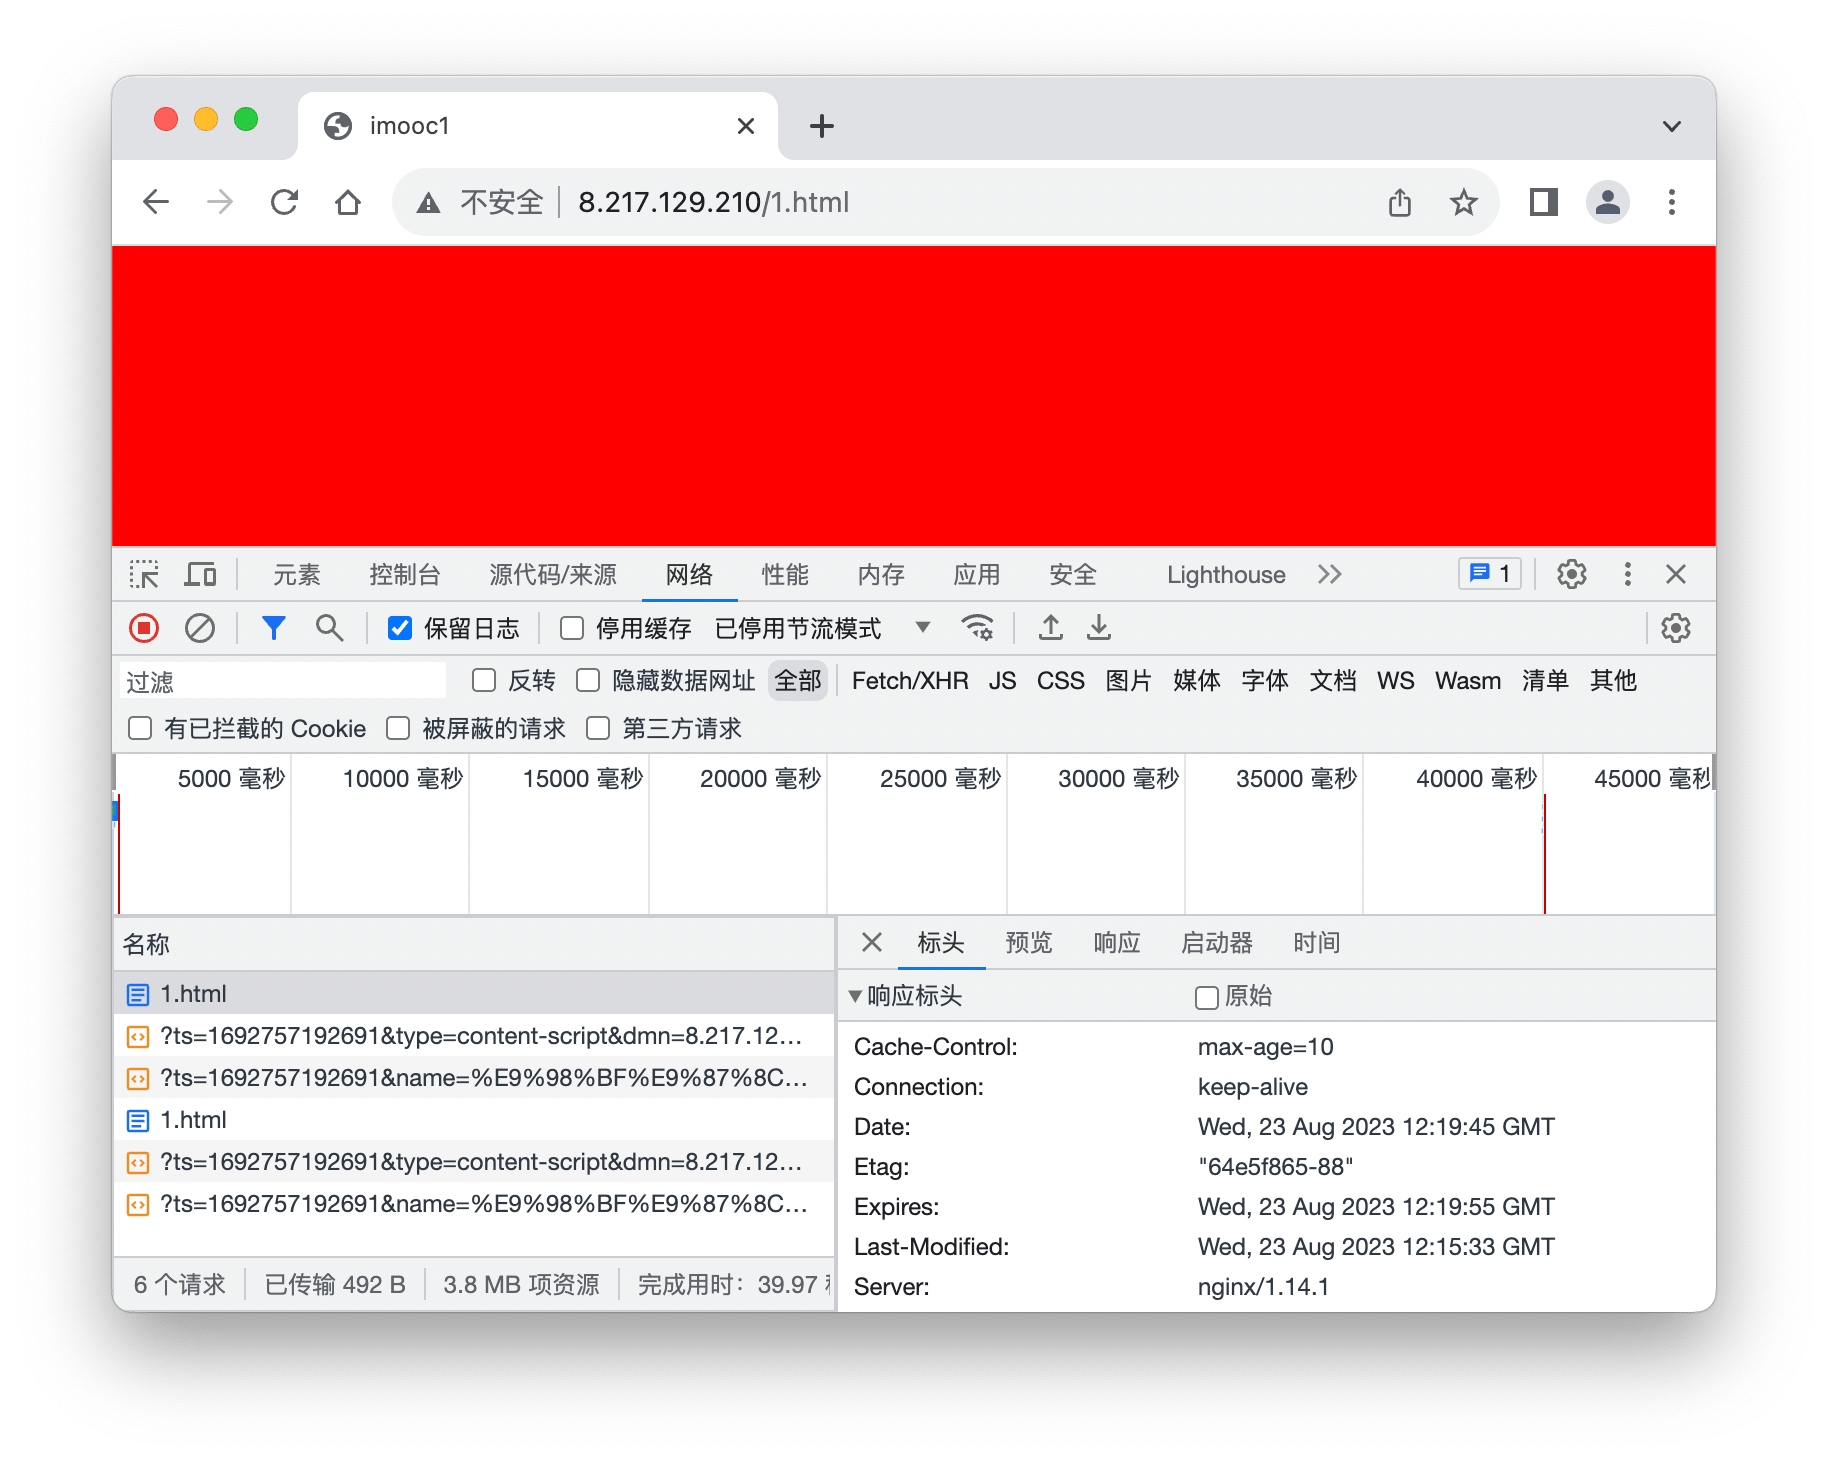
\includegraphics[width=1\textwidth]{./imgs/catch2023-08-23-20.21.19.png}
    \caption{缓存测试}
\end{figure}

参考:\href{https://blog.csdn.net/weixin_43834401/article/details/130599930}{nginx~-~Nginx配置浏览器缓存,页面展示更快一步}


\clearpage
\section{~nginx~代理服务}
% \colorbox{yellow}{\textbf{注:该板块的以下内容将}}

\subsection{~nginx~反向代理内涵}
正向代理与反向代理的区别:正向代理的服务对象是客户端。反向代理的服务对象是服务端。

\renewcommand{\figurename}{图} % 将图表的标题设置为中文“图”
\begin{figure}[htbp]
    \centering
    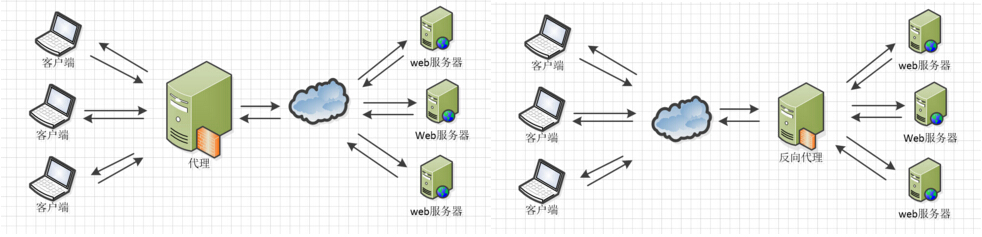
\includegraphics[width=1\textwidth]{./imgs/20160202133724350.jpg}
    \caption{引用\href{https://www.cnblogs.com/knowledgesea/p/5175711.html}{~cnblogs~-~Nginx配置详解}}
\end{figure}

\subsection{进行反代的准备工作}

了解nginx的语法规则
\renewcommand{\figurename}{图} % 将图表的标题设置为中文“图”
\begin{figure}[htbp]
    \centering
    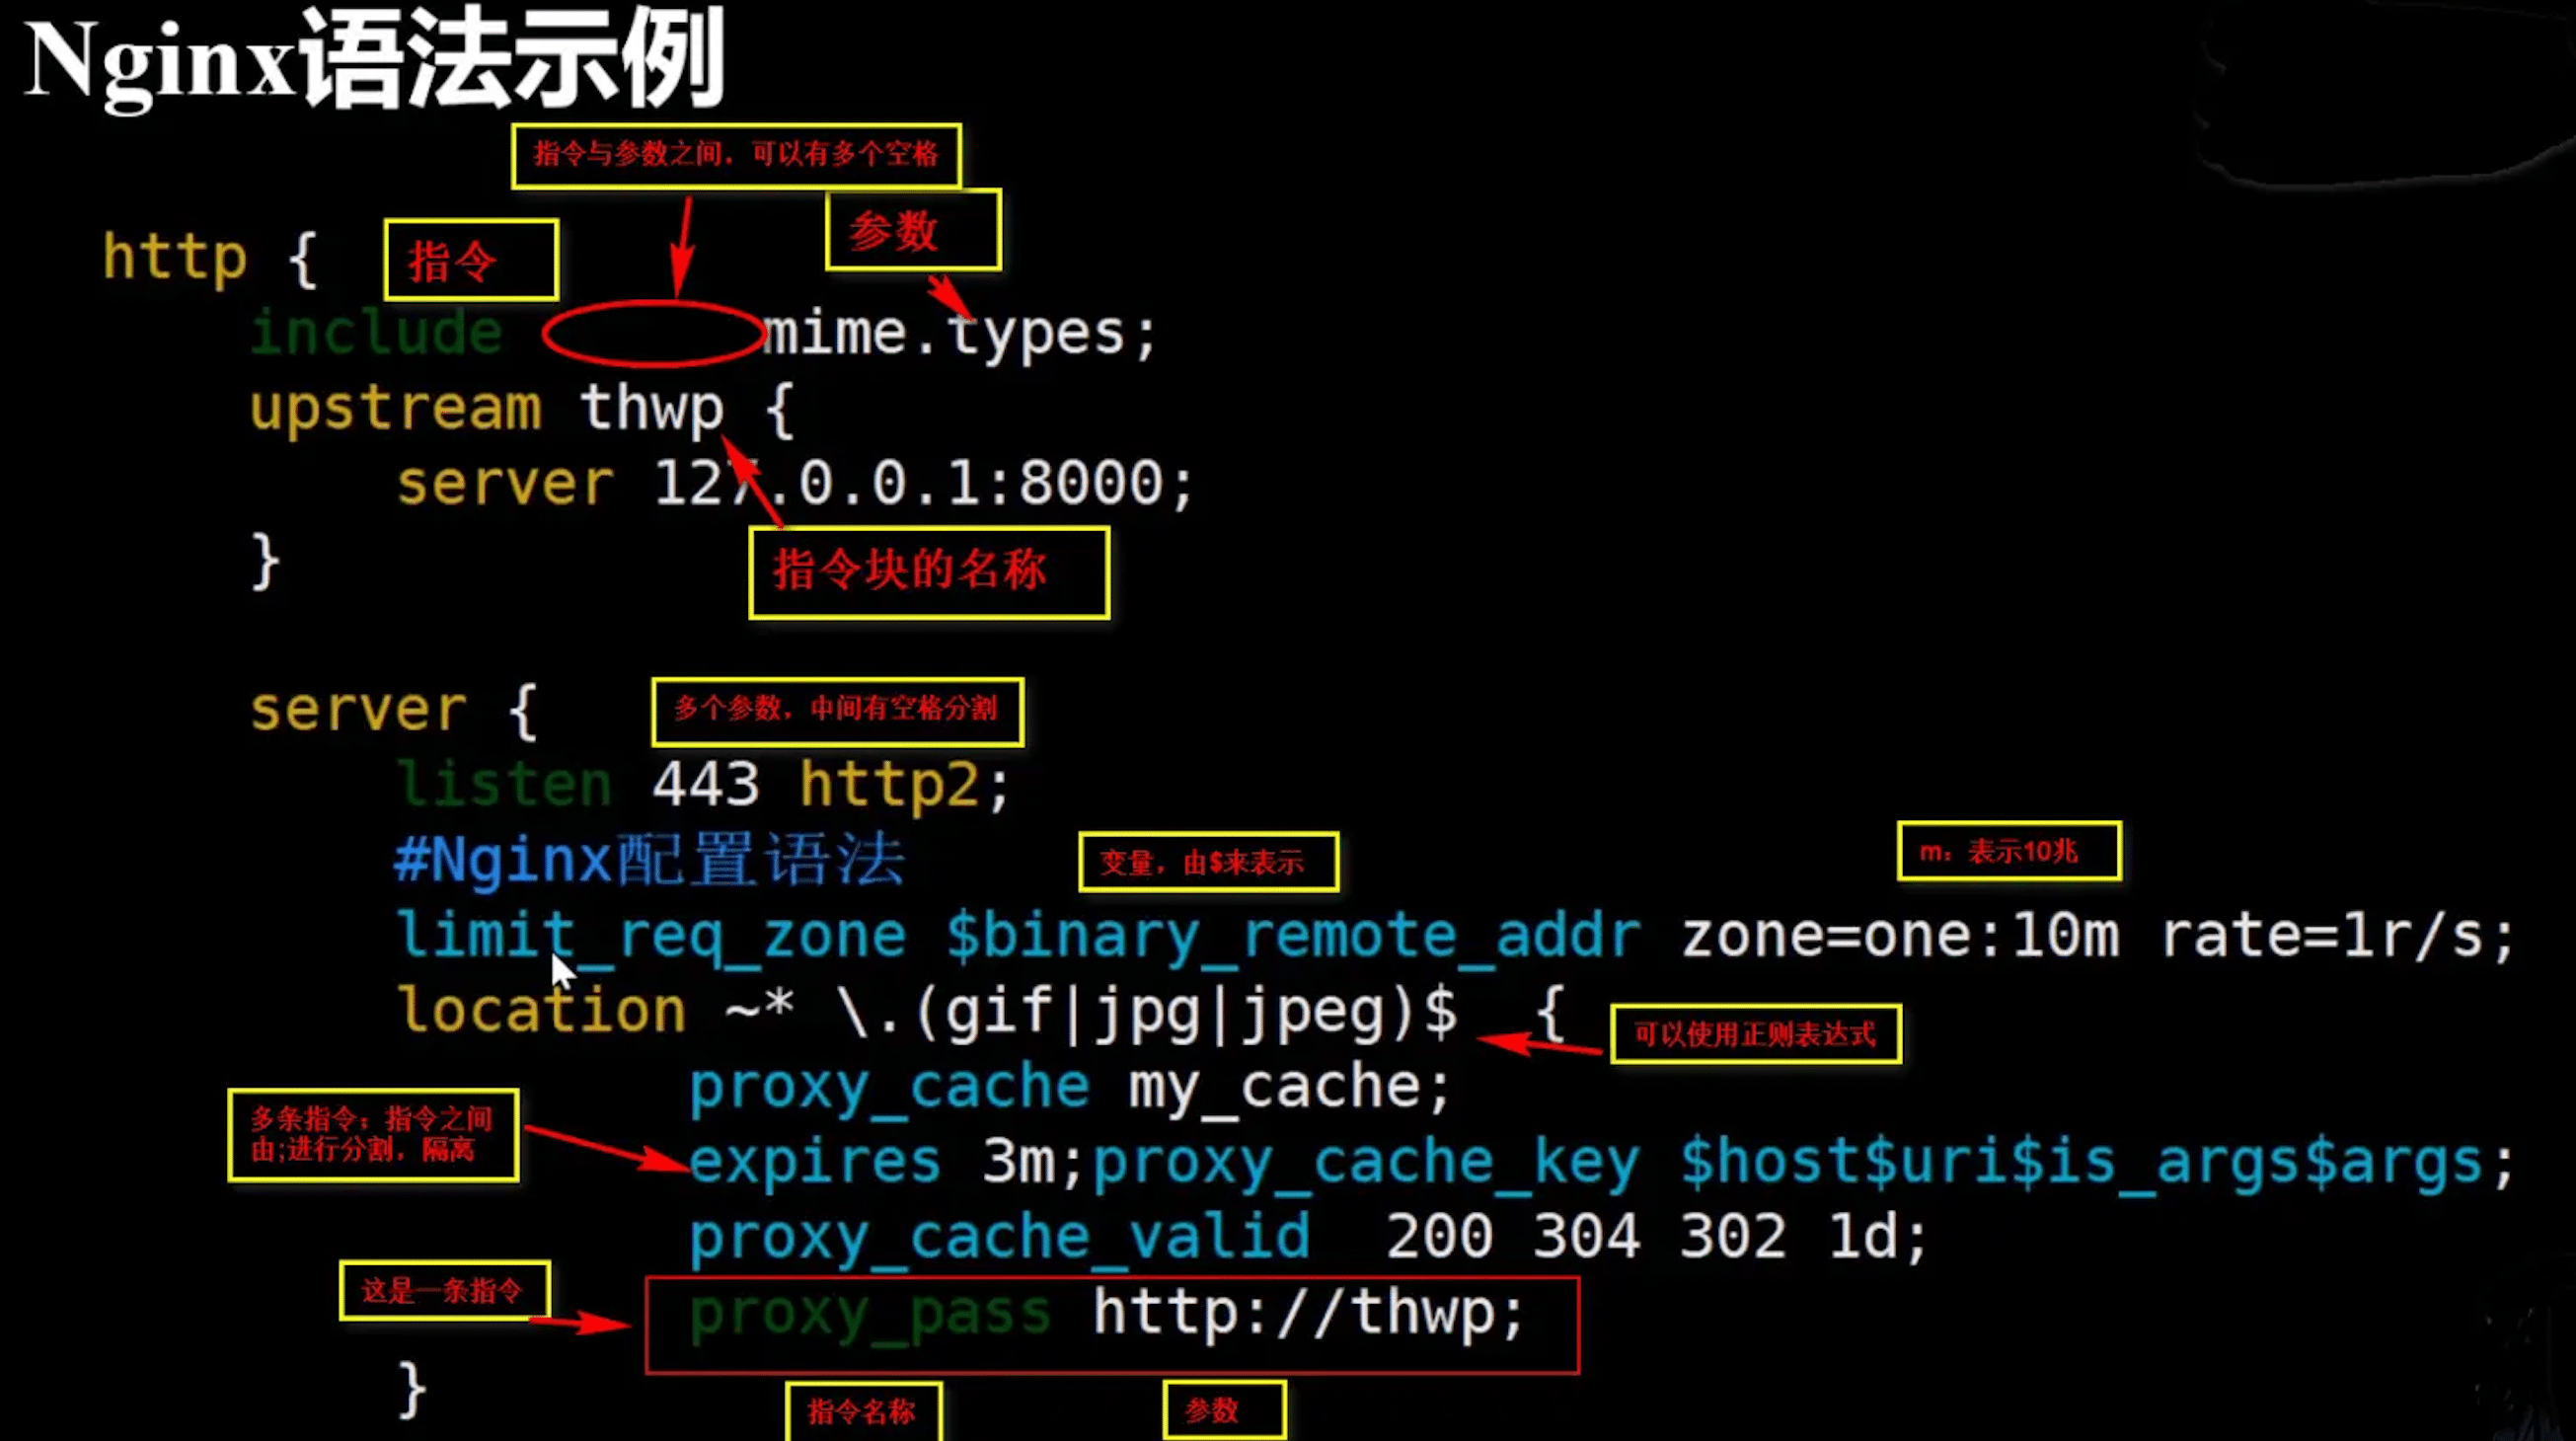
\includegraphics[width=0.8\textwidth]{./imgs/catch2023-08-25-00.46.05.png}
    \caption{语法规则}
\end{figure}

检查语法,查看当前系统中哪些进程正在监听与 Nginx 相关的端口。
\begin{lstlisting}
nginx -tc /etc/nginx/nginx.conf
netstat -luntp | grep nginx
\end{lstlisting}

\subsection{做两个配置文件}
我们做两个~/conf.d/xxx.conf~、~/conf.d/yyy.conf~来对配置反向代理。
\begin{itemize}
    \item xxx.conf~代表由~80~端口反代~8080~端口的内容,让~8080~端口的内容可以通过80端口访问。
    \item yyy.conf~是~8080~端口的正常网页内容的配置,在没有输入~8080~的条件下是不能进行访问的。
\end{itemize}

\subsubsection{xxx.conf}
首先创建~/etc/nginx/conf.d/xxx.conf~
\renewcommand{\lstlistingname}{配置代码} % 更改代码块标题的名称为 "Code"
\begin{lstlisting}[language=bash, caption=xxx.conf]
server {
    listen       80;
    server_name  8.217.129.210;
    access_log  /var/log/nginx/reverse_proxy.access.log  main;

    location / {
        root   /usr/share/nginx/html;
        index  index.html index.htm;
    }

    location ~ /y.html$ {
        proxy_pass http://127.0.0.1:8080;
    }

    error_page   500 502 503 504  /50x.html;
        location = /50x.html {
            root   /usr/share/nginx/html;
    }
}
\end{lstlisting}

\subsubsection{yyy.conf}
然后创建~/etc/nginx/conf.d/yyy.conf~
\renewcommand{\lstlistingname}{配置代码} % 更改代码块标题的名称为 "Code"
\begin{lstlisting}[language=bash, caption=yyy.conf]
server {
    listen       8080;
    server_name  8.217.129.210;

    access_log  /var/log/nginx/server.access.log  main;

    location / {
        root   /data/www/yyy;
        index  index.html index.htm;
    }

    error_page   500 502 503 504  /50x.html;
    location = /50x.html {
        root   /usr/share/nginx/html;
    }

}
\end{lstlisting}

创建反向代理测试目录及文件
\begin{lstlisting}
mkdir -p /data/www/yyy
vim /data/www/yyy/y.html
\end{lstlisting}
编辑y.html,保存并退出。
\begin{verbatim}
    <html lang="en">
    <head><meta charset="UTF-8" /></head>
        <body>
             <h1>测试反代访问</h1>
        </body>
    </html>
\end{verbatim}

\clearpage
\subsection{测试反代访问}
测试:~http://8.217.129.210/y.html~
\renewcommand{\figurename}{图} % 将图表的标题设置为中文“图”
\begin{figure}[htbp]
    \centering
    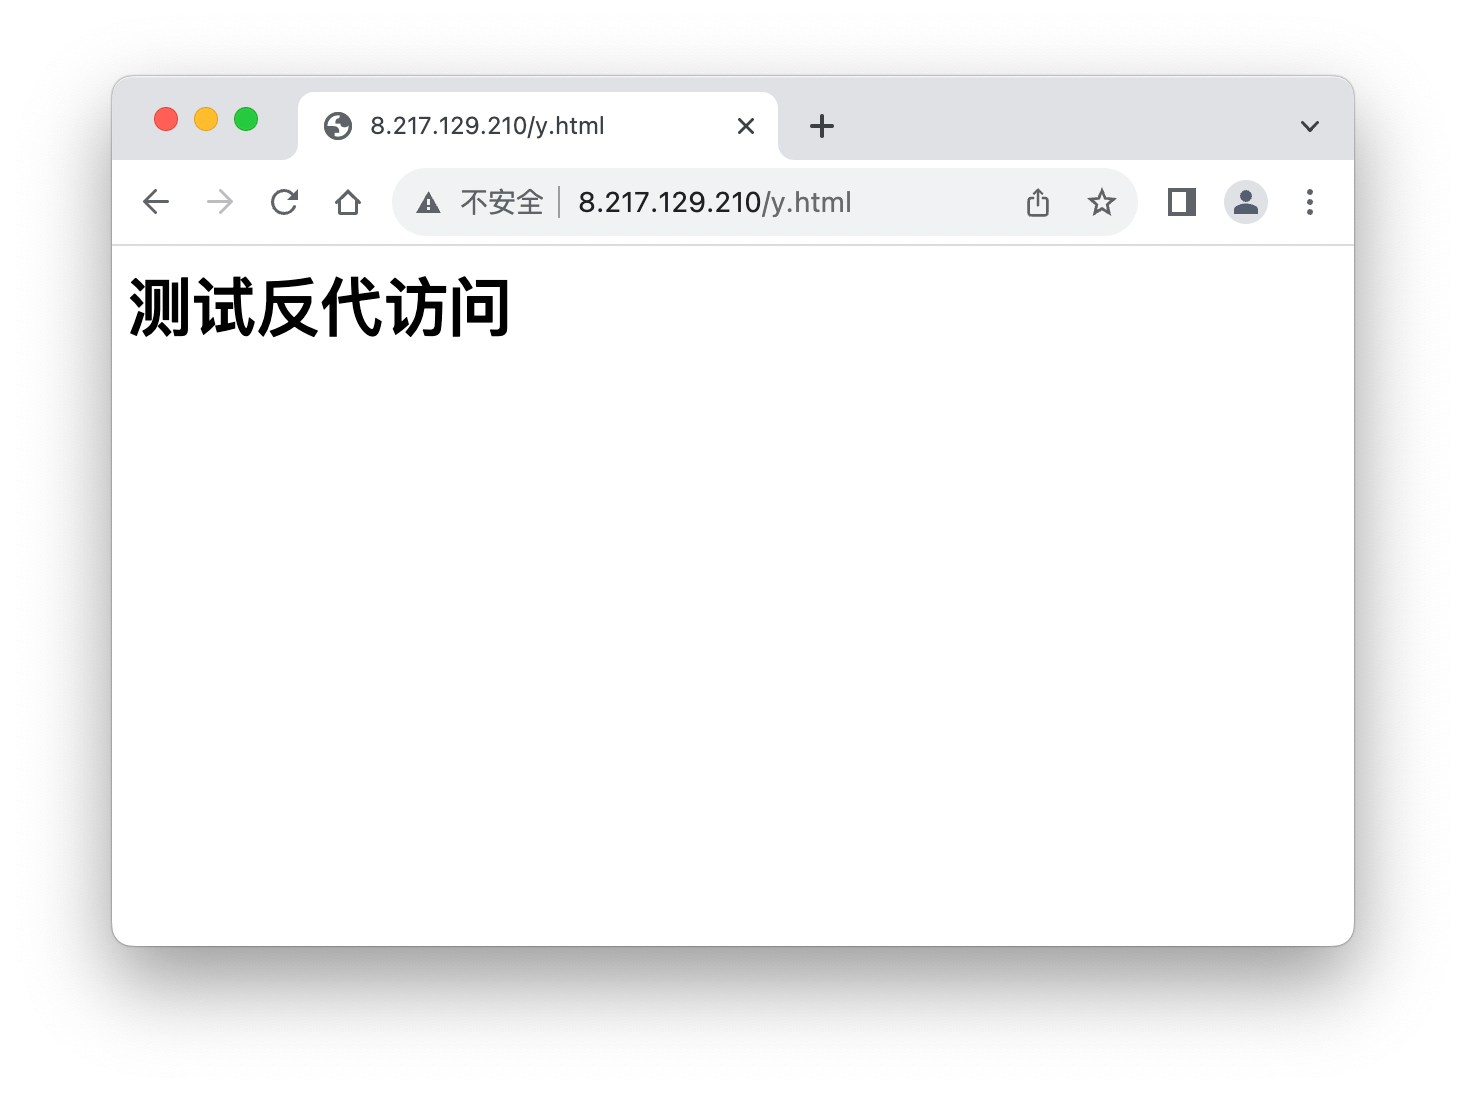
\includegraphics[width=0.6\textwidth]{./imgs/catch2023-08-25-08.52.45.png}
    \caption{反向代理测试}
\end{figure}

接着我们把~xxx.conf~配置的~8080~反代进行注释。
\begin{lstlisting}
location ~ /y.html$ {
     proxy_pass http://127.0.0.1:8080;
}
\end{lstlisting}

再测试反代访问
\renewcommand{\figurename}{图} % 将图表的标题设置为中文“图”
\begin{figure}[htbp]
\centering
\subfigure[注释前]{
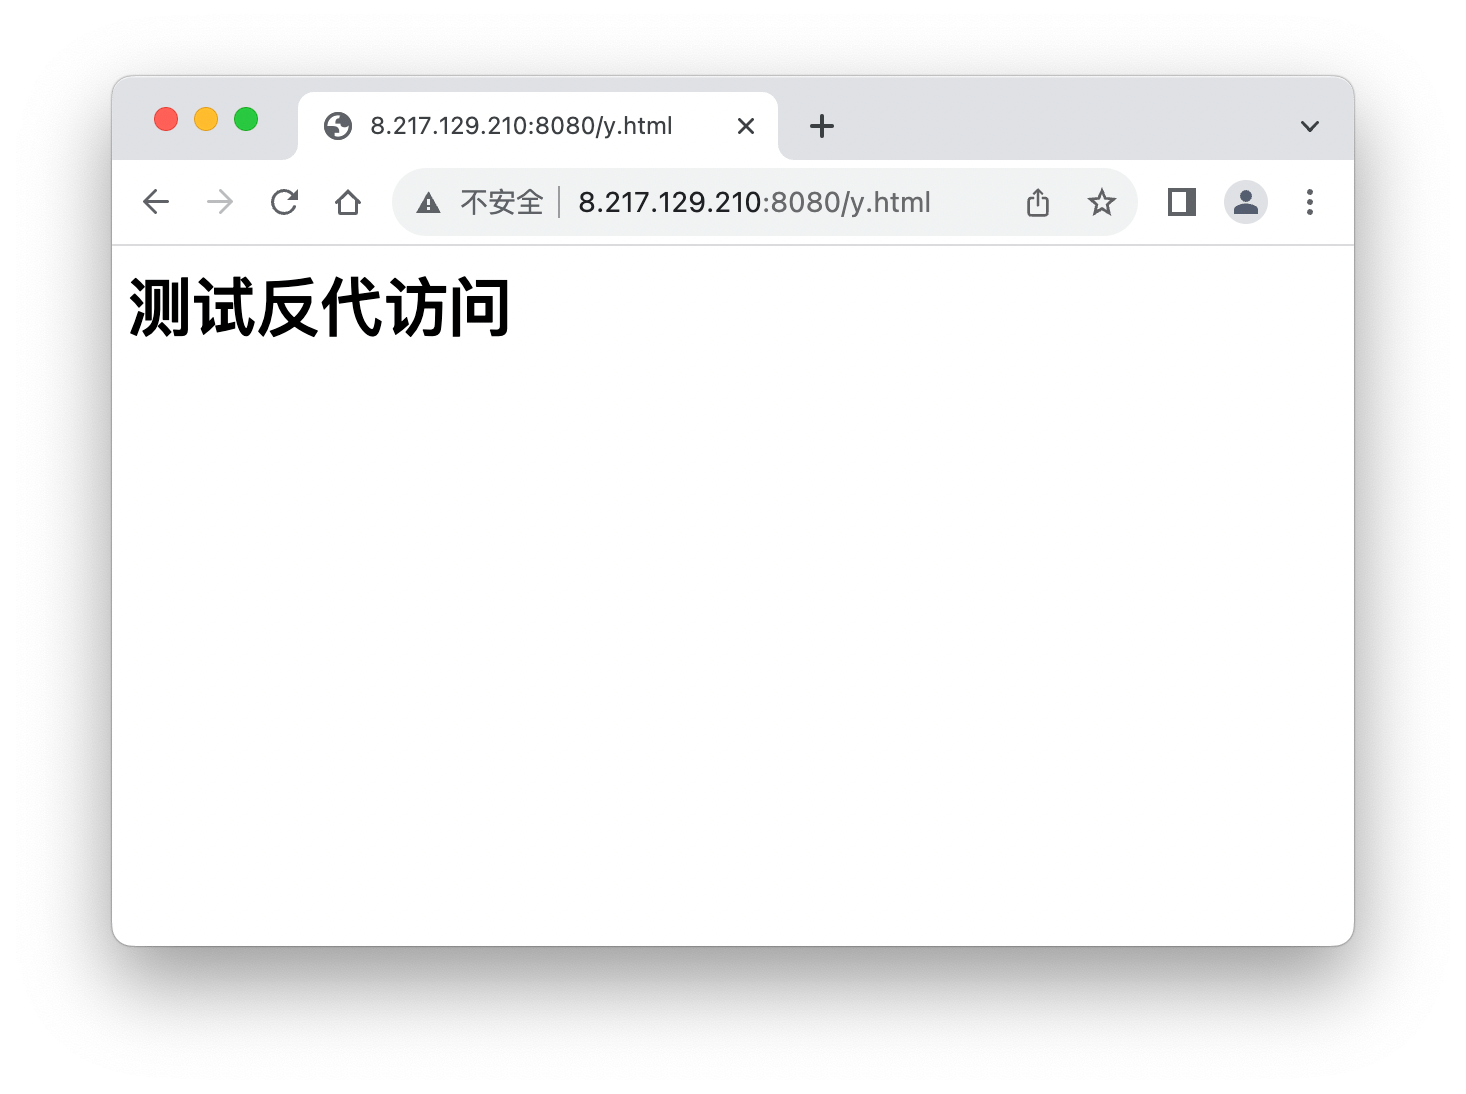
\includegraphics[width=0.47\textwidth]{./imgs/catch2023-08-25-09.26.21.png}
}
\subfigure[注释后]{
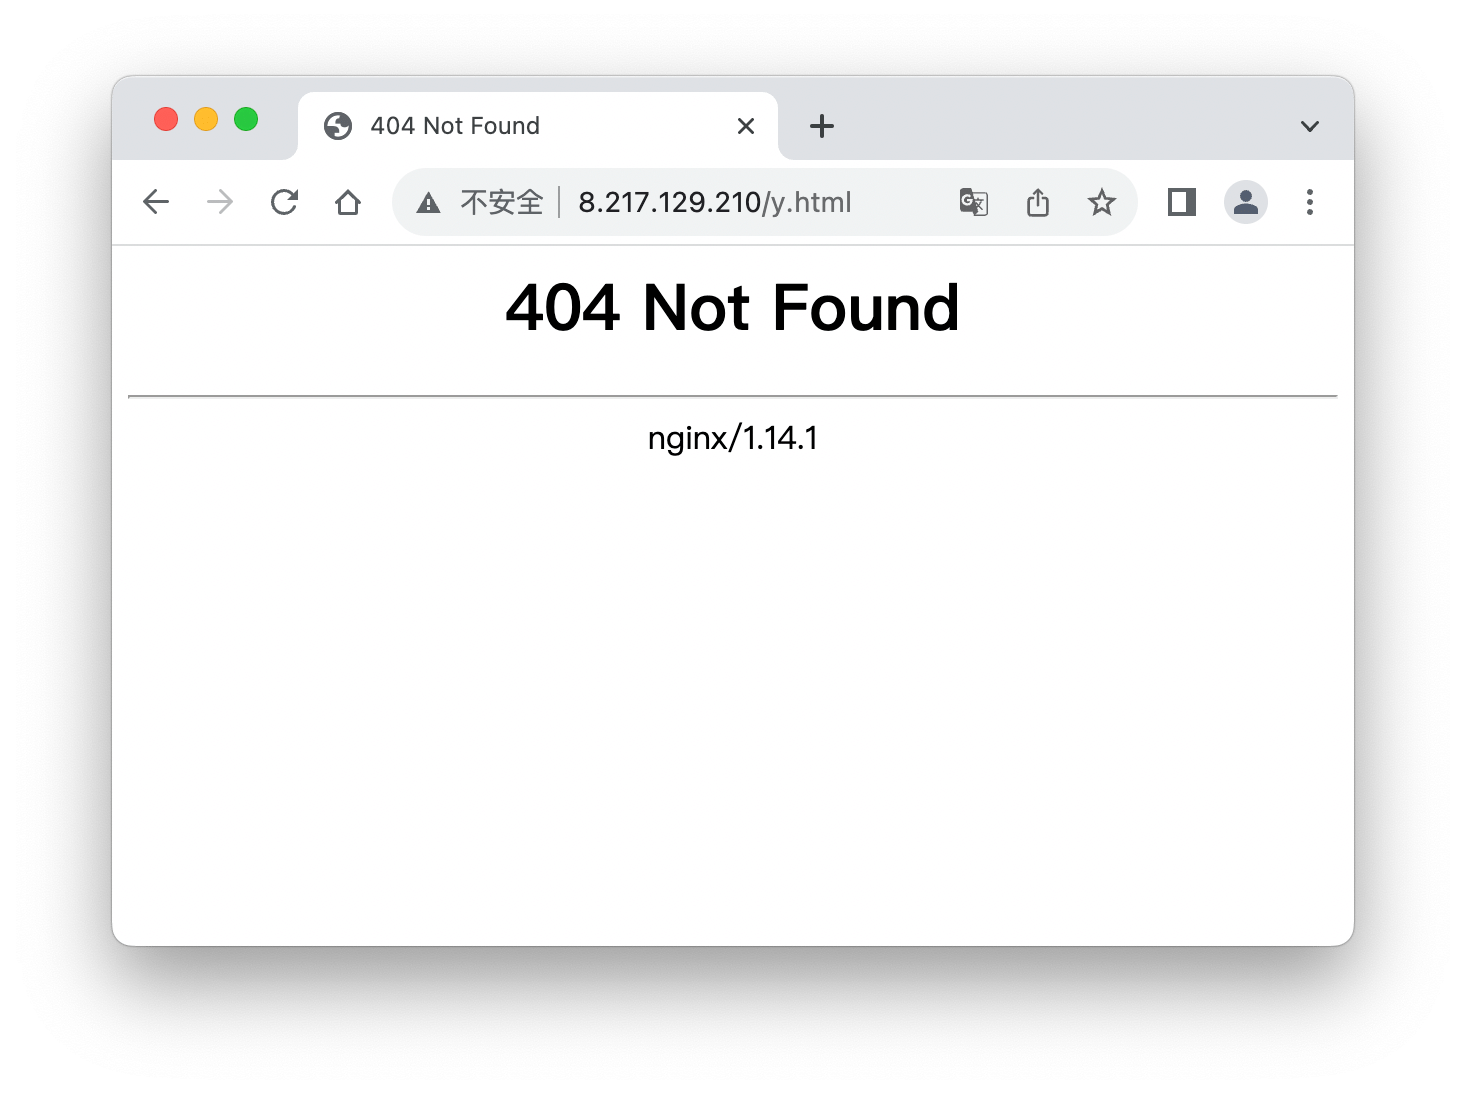
\includegraphics[width=0.47\textwidth]{./imgs/catch2023-08-25-09.26.09.png}
}
\centering
\end{figure}

\subsubsection{反代参考资料与正向代理扩展阅读}

反向代理参考资料:

\begin{itemize}
    \item \href{ https://www.jb51.net/article/220092.htm}{jb51~-~Nginx反向代理入门实战指南}
    \item \href{https://www.jb51.net/article/47722.htm}{jb51~-~常见的Nginx配置误区}
\end{itemize}

正向代理扩展阅读:

\begin{itemize}
    \item \href{https://bbs.huaweicloud.com/blogs/327420}{华为云~-~Linux安装Nginx}
    \item \href{https://access.redhat.com/documentation/zh-cn/red_hat_enterprise_linux/8/html/deploying_different_types_of_servers/setting-up-and-configuring-nginx_deploying-different-types-of-servers}{redhat~-~第2章~设置和配置 NGINX}
    \item \href{https://help.fanruan.com/finereport/doc-view-2644.html}{FineReport文档~-~Linux系统安装配置Nginx}
    \item \href{https://cloud.tencent.com/developer/article/1404153}{腾讯云~-~nginx添加第三方模块,以及启用nginx本身支持的模块}
    \item \href{http://www.nhooo.com/note/qacpfd.html}{nhooo~-~nginx安装第三方模块的方法}
    \item \href{https://www.jianshu.com/p/e265fc47eaa1}{简书~-~Nginx正向代理配置}
    \item \href{https://www.jianshu.com/p/48fd79a3cd23}{简书~-~nginx 安装详解(better version)}
\end{itemize}

\subsubsection{代理补充配置}

\begin{lstlisting}
location / {
    proxy_pass http://127.0.0.1:8080;
    proxy_redirect default;
    proxy_set_header Host $http_host;
    proxy_set_header x-Real-IP $remote_addr;
    proxy_connect_timeout 30;
    proxy_send_timeout 60;
    proxy_read_timeout 60;
    proxy_buffer_size 32k;
    proxy_buffering on;
    proxy_buffers 4 128k;
    proxy_busy_buffers_size 256k;
    proxy_max_temp_file_size 256k;
}
\end{lstlisting}

\clearpage
\section{负载均衡应用场景}

\begin{figure}[htbp]
    \centering
    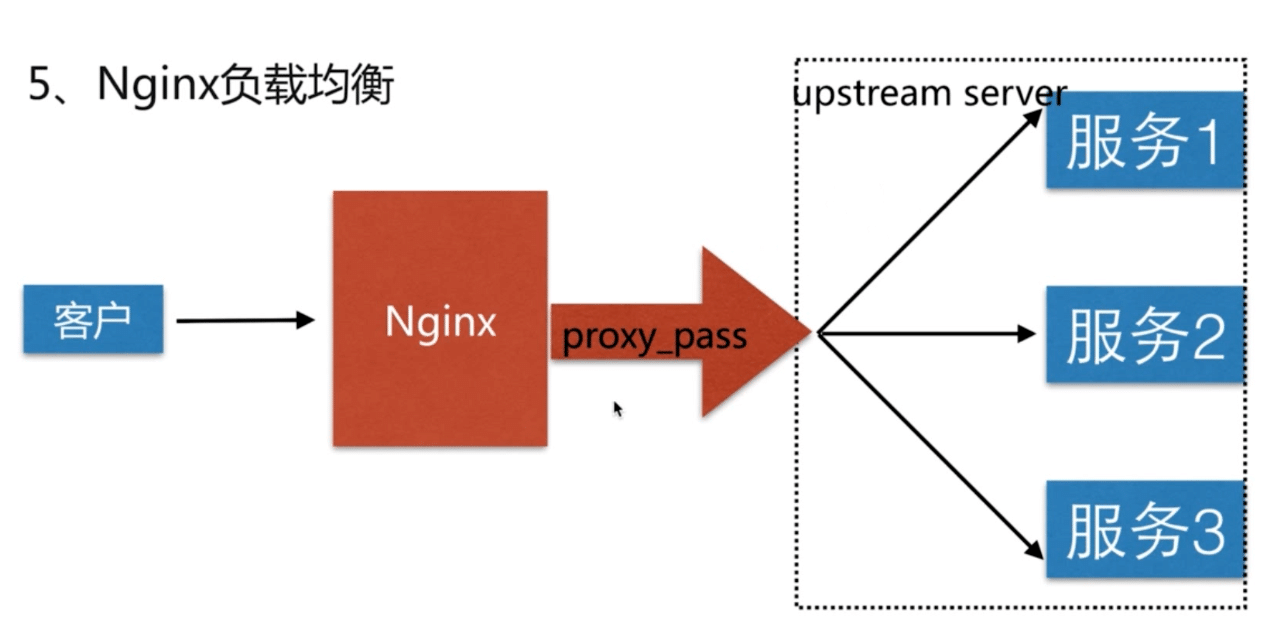
\includegraphics[width=0.6\textwidth]{./imgs/catch2023-08-25-22.40.09.png}
    \caption{反向代理测试}
\end{figure}

\subsection{负载均衡的准备工作}

创建配置文件,以此创建server2、server3的配置文件。
\begin{lstlisting}
touch /etc/nginx/conf.d/server1.conf
\end{lstlisting}

编辑配置server1.conf文件,server2.conf、server3.conf~对应目录~/data/code2,\\
/data/code3,端口对应~8002,~8003,日志文件~server1.access.log~同理。
\begin{lstlisting}
server {
    listen       8001;
    server_name  localhost;

    #charset koi8-r;
    access_log  /var/log/nginx/server1.access.log  main;

    location / {
        root   /data/code1;
        index  index.html index.htm;
    }
    error_page   500 502 503 504 404  /50x.html;
    location = /50x.html {
        root   /usr/share/nginx/html;
    }
}
\end{lstlisting}

创建并编辑~/data/code1/index.html,以此类推创建~/data/code2/index.html,\\
~/data/code3/index.html。
\begin{verbatim}
    <html>
    <head>
        <meta charset="utf-8">
        <title>server1</title>
    </head>
    <body style="background-color:yellow;">
        <h1>Server 1<h1>
    </body>
    </html>
\end{verbatim}

\verb|systemctl start nginx|~,以IP加端口的方式访问。

\begin{figure}[htbp]
    \centering
    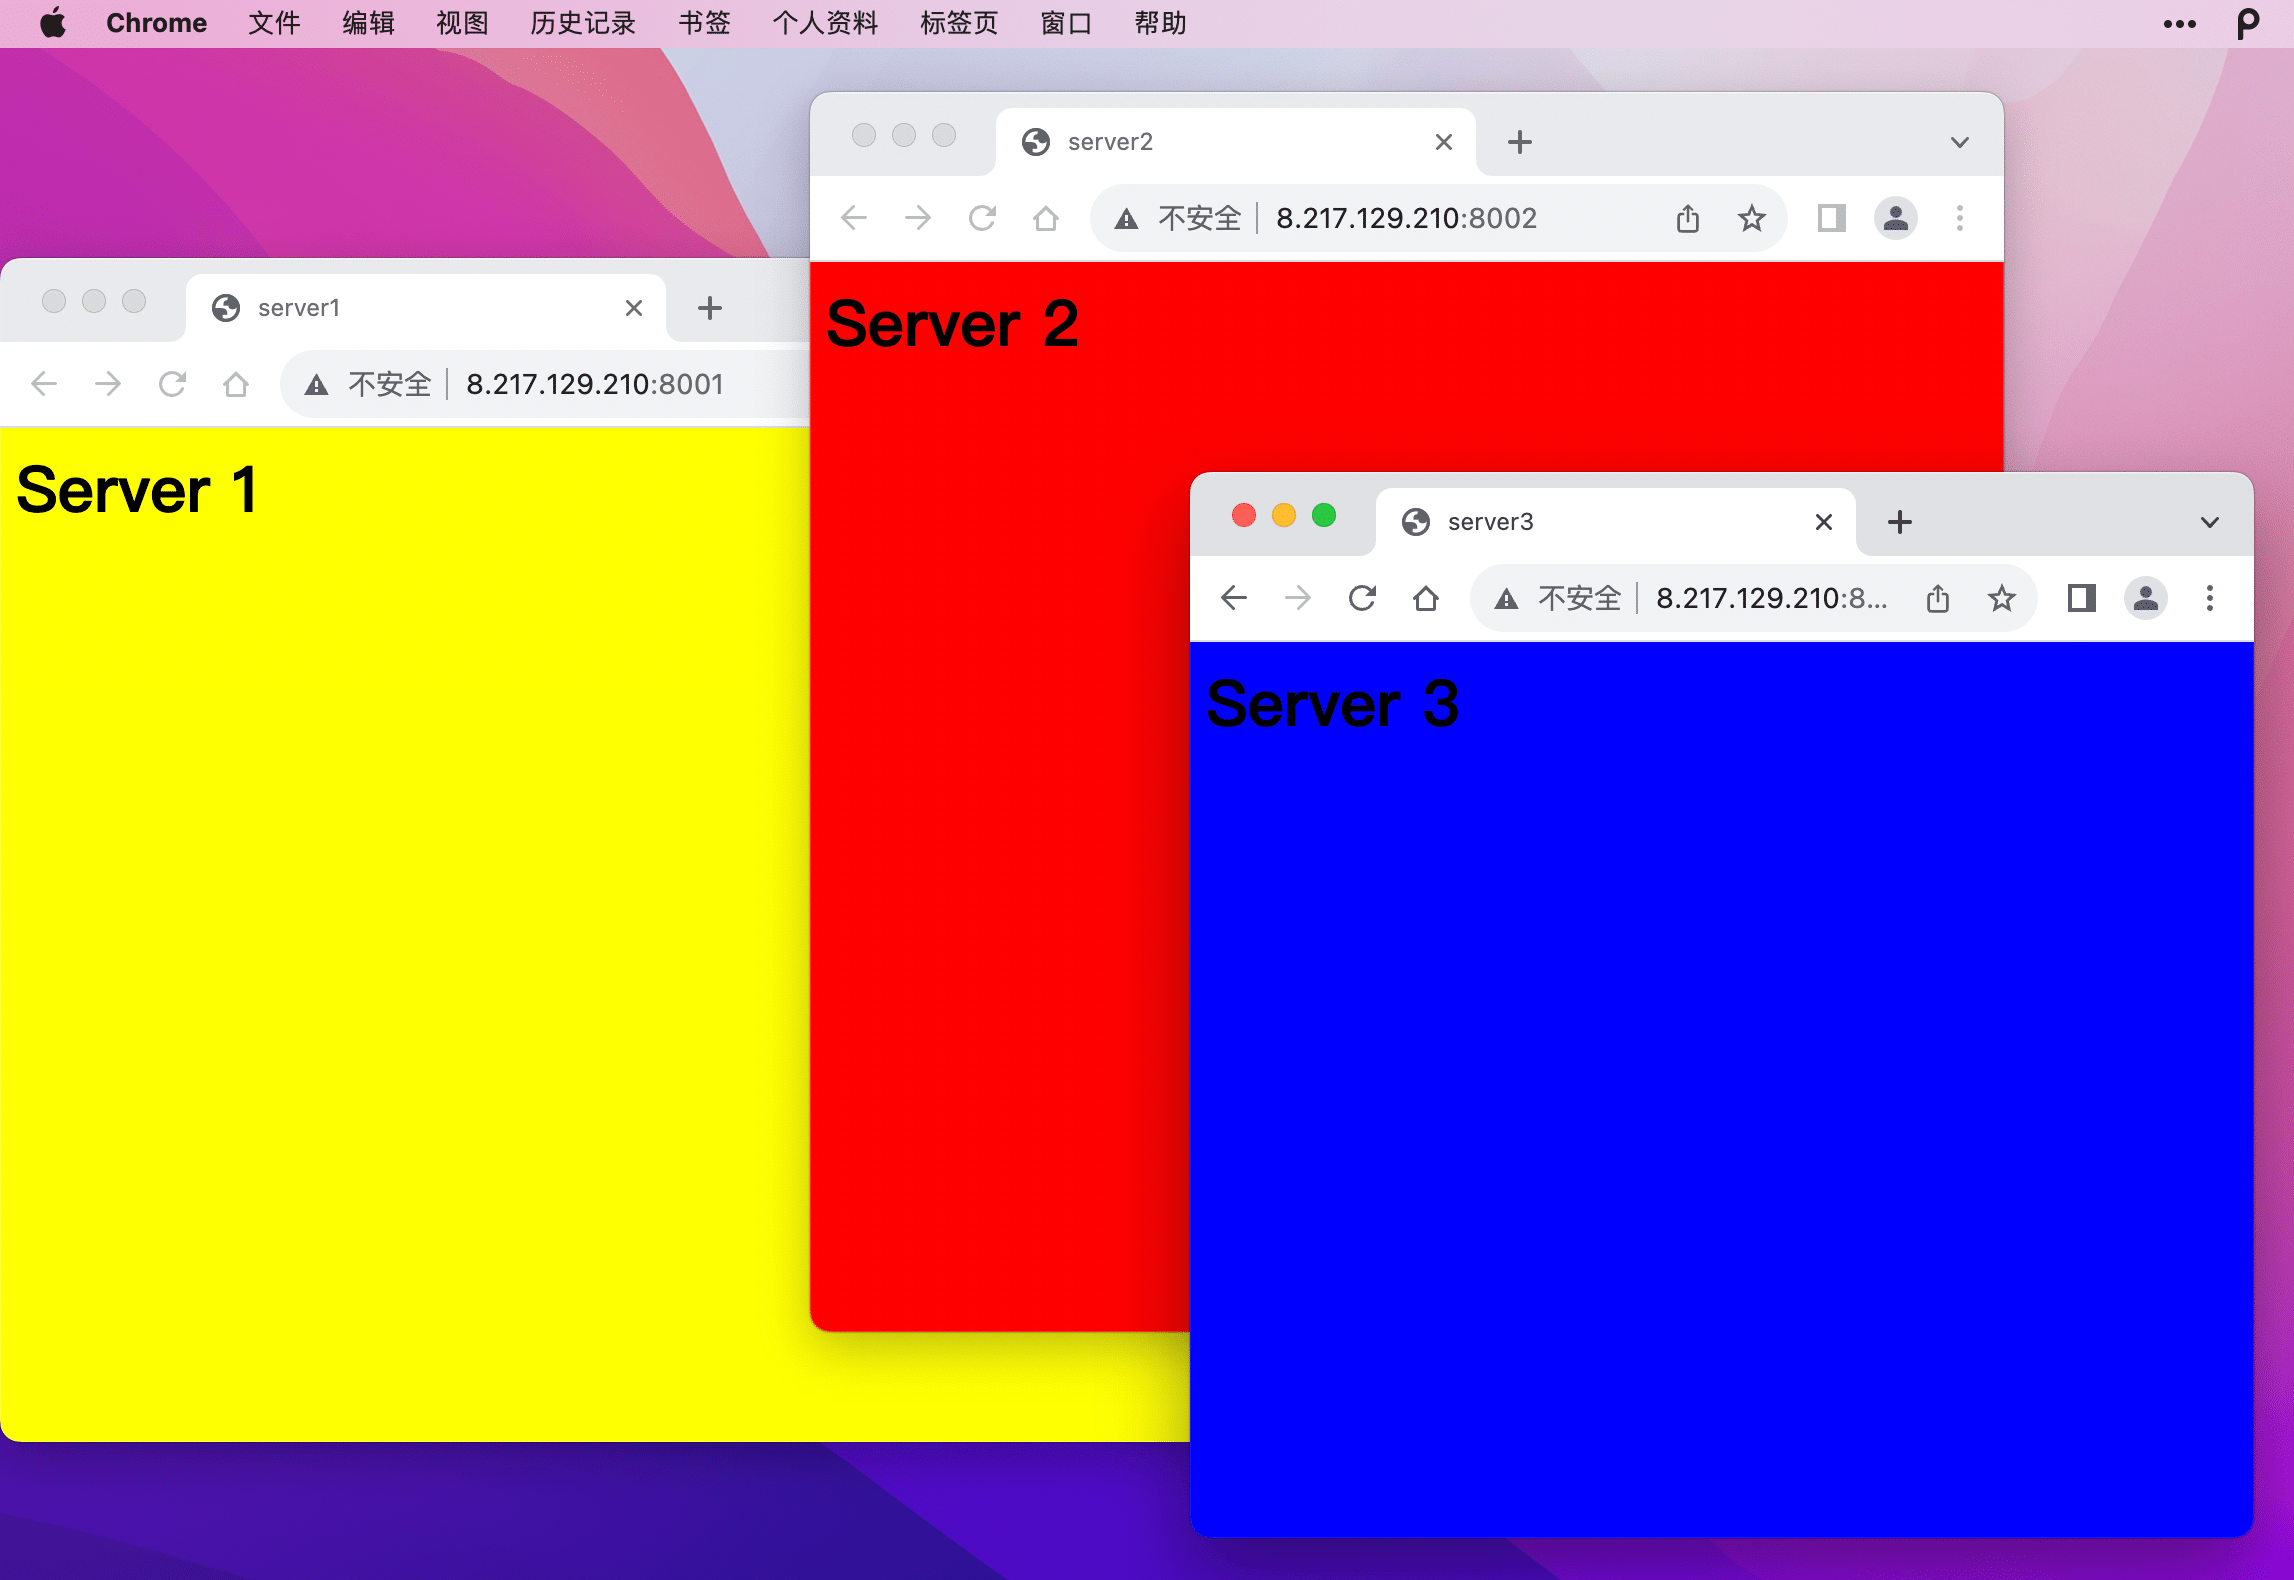
\includegraphics[width=0.6\textwidth]{./imgs/catch2023-08-26-10.43.17.png}
    \caption{准备工作测试}
\end{figure}

\subsection{负载均衡配置}
\verb|vim /etc/nginx/conf.d/upstream_test.conf|~接下来以负载均衡的方式访问,以一个地址负载到不同的服务器上。

\begin{lstlisting}
upstream test {
    server 8.217.129.210:8001;
    server 8.217.129.210:8002;
    server 8.217.129.210:8003;
}

server {
    listen       80;
    server_name  8.217.129.210;
    access_log  /var/log/nginx/test_proxy.access.log  main;
    resolver  1.1.1.1;

    location / {
        include proxy_params;
        proxy_pass http://test;
    }

    error_page   500 502 503 504  /50x.html;
    location = /50x.html {
        root   /usr/share/nginx/html;
    }
}
\end{lstlisting}

\subsection{负载均衡配置解读}

\subsubsection{nginx:[emerg] open()“/etc/nginx/proxy\_params” failed (2: No such file or directory)}

方案一:将~include proxy\_params; 替换为

\begin{lstlisting}
proxy_set_header Host $http_host;
proxy_set_header X-Real-IP $remote_addr;
proxy_set_header X-Forwarded-For $proxy_add_x_forwarded_for;
proxy_set_header X-Forwarded-Proto $scheme;
\end{lstlisting}

方案二:vim /etc/nginx/proxy\_params~文件

\begin{lstlisting}
proxy_set_header Host $http_host;
proxy_set_header X-Real-IP $remote_addr;
proxy_set_header X-Forwarded-For $proxy_add_x_forwarded_for;
proxy_set_header X-Forwarded-Proto $scheme;
\end{lstlisting}

\begin{enumerate}
    \item \verb|proxy_set_header Host $http_host;|~把客户端请求中的 Host 头部信息传递给后端服务器。
    \verb|$http_host| 变量是客户端请求中的 Host 头部的值。
    \item \verb|proxy_set_header X-Real-IP $remote_addr;|~把客户端请求的真实 IP 地址传递给后端服务器。
    \item \verb|proxy_set_header X-Forwarded-For $proxy_add_x_forwarded_for;|\\这个指令将会把客户端请求的真实~IP~地址传递给后端服务器。
    \item \verb|proxy_set_header X-Forwarded-Proto $scheme;|~把客户端请求的协议类型传递给后端服务器。
\end{enumerate}

以上参考:\href{https://www.jianshu.com/p/0e0cf88da24e}{负载均衡/etc/nginx/proxy\_params报错}

\subsubsection{upstream test~与~http://test~的联系}

其中~http://test~是一个upstream,upstream是nginx的一个模块,用来配置负载均衡的服务器列表。 参考:\href{https://blog.csdn.net/weixin_44623055/article/details/124715177}{Nginx~-~Nginx负载均衡}

\begin{lstlisting}
upstream test {
    server 8.217.129.210:8001;
    server 8.217.129.210:8002;
    server 8.217.129.210:8003;
}

server {
    ...
location / {
    include proxy_params;
    proxy_pass http://test;
}
    ...
}
\end{lstlisting}

\clearpage
再检查一遍~\verb|nginx -tc /etc/nginx/nginx.conf|,并重启~nginx~服务 \\ \verb|systemctl reload nginx|。

这个时候我们假定某个服务down了,剩下两个服务是否可用,利用~iptables~拒绝掉~8002~端口配置。
\begin{lstlisting}
iptables -I INPUT -p tcp --dport 8001 -j DROP
\end{lstlisting}
还原之前的~iptables~策略
\begin{lstlisting}
iptables -D INPUT -p tcp --dport 8001 -j DROP
iptables -F
\end{lstlisting}

从下图我们可以观察到刷新一遍会发现,每次访问的服务器端口都不一样,nginx检测到server1不能用时会在server2、server3来回跳转。

\begin{figure}[htbp]
    \centering
    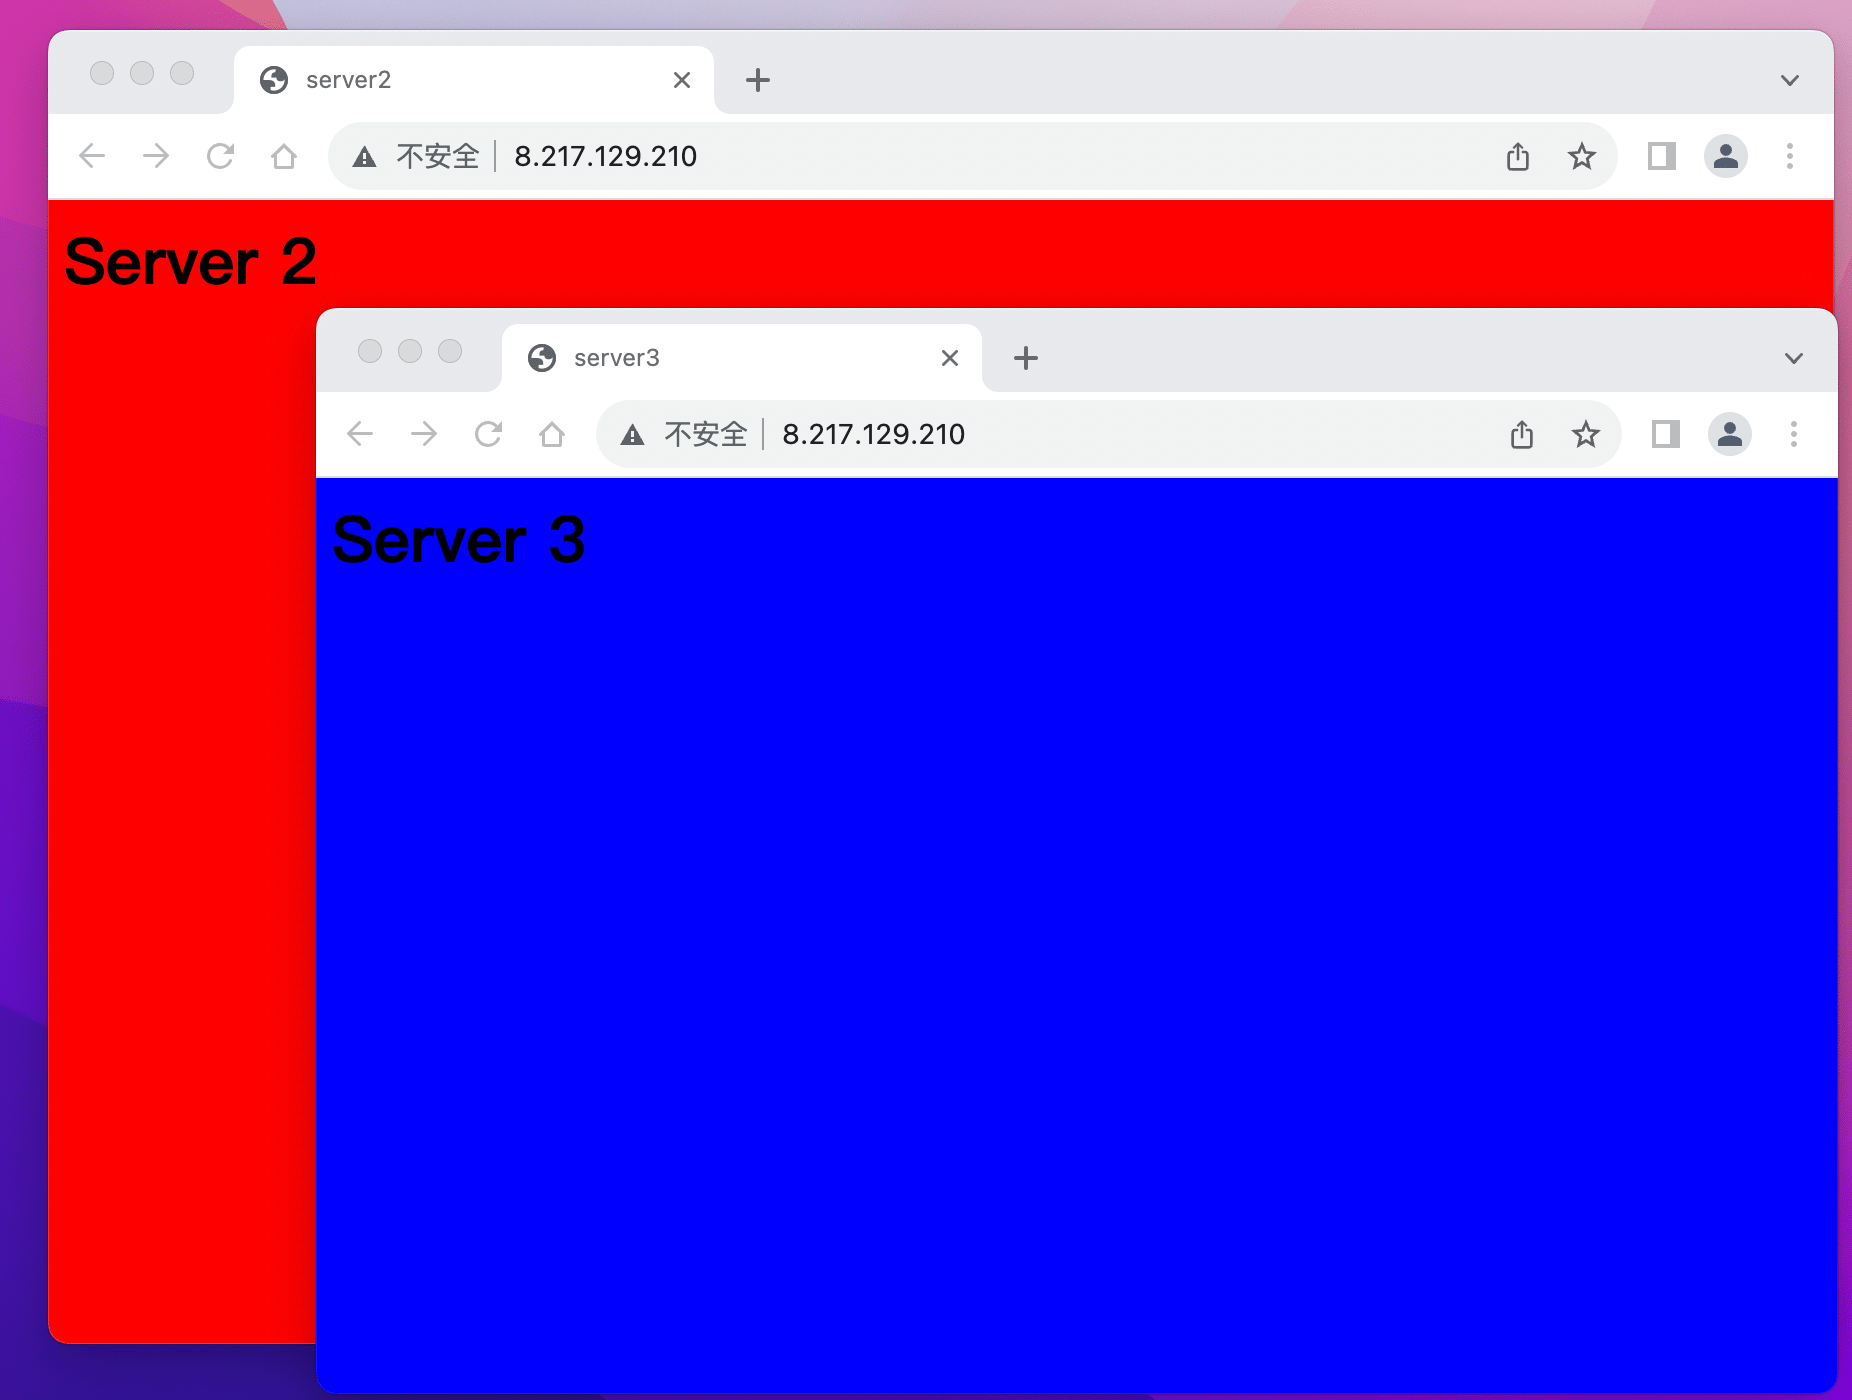
\includegraphics[width=0.6\textwidth]{./imgs/catch2023-08-26-12.39.02.png}
    \caption{负载均衡测试}
\end{figure}

\begin{itemize}
    \item \href{https://tamerlan.dev/how-to-set-up-nginx-load-balancing-a-step-by-step-guide/}{How to Set Up NGINX Load Balancing: A Step-by-Step Guide}
    \item \href{https://upcloud.com/resources/tutorials/configure-load-balancing-nginx}{How to configure load balancing using Nginx}
\end{itemize}

\clearpage
\section{nginx~缓存的使用}
nginx发送请求给服务器,并且生成了一定量的缓存文件,客户端发出了请求,nginx检查出自己对应的缓存文件,不在向服务端进行请求,而是直接返回缓存的内容给客户端。

\begin{itemize}
    \item \href{https://www.cnblogs.com/itzgr/p/13321980.html}{cnblogs~-~009.Nginx缓存配置}
    \item  \href{https://juejin.cn/post/7079601613135937550}{juejin~-~Nginx配置前端http缓存}
\end{itemize}



\subsection{proxy\_cache~配置}

\begin{enumerate}
    \item 语法:proxy\_cache zone | off;
    \item 默认:proxy\_cache off;
    \item 可配置段:http、server、location
    \item 作用:设置是否开启对后端响应的缓存,如果开启,参数值就是zone的名称。
\end{enumerate}

\begin{lstlisting}
proxy_cache mycache;
\end{lstlisting}

\subsection{proxy\_cache\_path~配置}

\begin{enumerate}
    \item 缓存目录:/data/nginx/cache
    \item 缓存名称:one,且占用内存~10M;缓存目录级别为2。
    \item 缓存最大时间为~60~分钟,加载器每次迭代过程最多执行~300~毫秒。
    \item 每次迭代过程中最多加载~200~个文件,缓存硬盘空间最多为~200M。
    \item 注意:缓存位置是一个目录应该先创建好,nginx并不会帮我们创建这个缓存目录。
\end{enumerate}

\begin{lstlisting}
proxy_cache_path /data/nginx/cache  \
keys_zone=one:10m levels=1:2 \
inactive=60m loader_threshold=300 \
loader_files=200 max_size=200m;
\end{lstlisting}

\subsection{proxy\_cache\_path~的使用}
使用名称为one的缓存,缓存有效期为1分钟,被请求3次以上时才缓存。
\begin{lstlisting}
http{
    proxy_cache_path /data/nginx/cache  \
    keys_zone=one:10m levels=1:2 \
    inactive=60m loader_threshold=300 \
    loader_files=200 max_size=200m;
    server {
        listen 8080;
        proxy_cache one;
        location / {
            proxy_pass http://backend1;
        }
        location /some/path {
            proxy_pass http://backend2;
            proxy_cache_valid any 1m;
            proxy_cache_min_uses 3;
            proxy_cache_bypass $cookie_nocache $arg_nocache $arg_comment;
        }
    }
}
\end{lstlisting}

\verb|proxy_cache_bypass $cookie_nocache $arg_nocache$arg_comment;| 我们不知道意思,但可以通过官网进行查阅。

\begin{enumerate}
    \item \url{https://nginx.org/en/docs/http/ngx_http_proxy_module.html}
    \item \url{https://nginx.org/en/docs/varindex.html}
\end{enumerate}

以及其他

\begin{enumerate}
    \item \url{https://www.cnblogs.com/tkzc2013/p/14255645.html}
    \item \url{https://www.cnblogs.com/konglxblog/p/16485641.html}
\end{enumerate}

\clearpage
\section{附录}
\subsection{Nginx~动静分离}
为了提高网站的响应速度,减轻程序服务器的负载,对于静态资源,如~images,~js,~css~等文件,可以在反向代理服务器中进行缓存,这样浏览器在请求一个静态资源时,
代理服务器就可以直接处理,而不用将请求转发给后端服务器。对于用户请求的动态文件,如~jsp,则转发给~Tomcat~服务器处理,这就是动静分离。
即动态文件与静态文件的分离。

参考:

\begin{itemize}
    \item \href{https://www.jianshu.com/p/6c1a230f9e26}{11.Nginx动静分离配置}
    \item \href{}{text}
\end{itemize}

\subsection{nginx~重写}
rewrite功能就是,使用nginx提供的全局变量或自己设置的变量,结合正则表达式和标记位实现URL重写以及重定向。比如:更换域名后需要保持旧的域名能跳转到新的域名上、
某网页发生改变需要跳转到新的页面、网站防盗链等等需求。

参考:\href{https://blog.csdn.net/Moshizhu/article/details/125136067}{csdn~-~Nginx~重写}

\subsection{~nginx~相关教程}
\begin{enumerate}
    \item 淘宝核心系统服务器平台组成员 - Nginx入门指南:\url{https://doc.yonyoucloud.com/doc/wiki/project/nginx/index.html}
    \item aceld nginx:\url{https://aceld.gitbooks.io/nginx-zh/content/nginx.html}
    \item ~nginx~开发从入门到精通:\url{https://www.kancloud.cn/kancloud/master-nginx-develop/51800}
    \item ~老马啸西风~-~nginx~教程:\url{https://houbb.github.io/2018/11/22/nginx-01-overview-01}
    \item NGINX 完全手册:\url{https://www.freecodecamp.org/chinese/news/the-nginx-handbook/#how-to-use-nginx-as-a-load-balancer}
\end{enumerate}

\subsection{~nginx~工作上的例子}
\begin{enumerate}
    \item 工作中nginx整理:\url{https://www.cnblogs.com/windysai/p/14122105.html}
    \item 关于Nginx,在日常工作中你可能用到的操作就这些了:\url{https://juejin.cn/post/7071846058447339527}
    \item 工作必会的Nginx启动安装命令和常用配置例子:\url{https://www.modb.pro/db/87890}
    \item 深入~Nginx~之配置篇:\url{https://learnku.com/articles/24795}
    \item NGINX 从入门到精通,学会这些就够了:\url{https://learnku.com/articles/46237}
\end{enumerate}

\subsection{~nginx~典型应用场景}
\begin{enumerate}
    \item https://juejin.cn/s/nginx典型应用场景
    \item 全面了解Nginx主要应用场景:\url{https://cloud.tencent.com/developer/article/1943958}
    \item 都在用Nginx,你真的知道它的应用场景吗?:\url{https://blog.51cto.com/u_14153136/3241717}
    \item 彻底搞懂 Nginx 五大应用场景!出去吹牛逼再也不担心了:\url{https://segmentfault.com/a/1190000040420111}
\end{enumerate}

\subsection{~mysql~必知必会}
\begin{enumerate}
    \item https://awesome-programming-books.github.io/mysql/MySQL必知必会.pdf
    \item \url{https://cfangxu-2.gitbook.io/front-end-basics/gong-ju-lei/mysql/mysql}
    \item \url{https://www.modb.pro/db/97783}
\end{enumerate}


\end{CJK*}
\end{document}
